\section{Hiện thực và đánh giá}
\subsection{Khởi tạo Keycloak realm}
\begin{itemize}
    \item \textbf{Mục tiêu}: Cung cấp một luồng xác thực tập trung, trong đó Keycloak đóng vai trò Identity Provider (IdP) còn Cloudflare Access đóng vai trò lớp kiểm soát truy cập ở biên mạng.
    \item \textbf{Phạm vi}: Thử nghiệm trên môi trường sử dụng \texttt{trycloudflare} để công bố tạm thời dịch vụ Keycloak ra Internet phục vụ quá trình tích hợp và đánh giá.
    \item \textbf{Kết quả mong đợi}: Người dùng phải đăng nhập qua Keycloak trước khi được Cloudflare cấp quyền truy cập ứng dụng được bảo vệ.
\end{itemize}

\subsection{Khởi chạy \texttt{trycloudflare} để công bố Keycloak}
Giai đoạn đầu tiên là đưa dịch vụ Keycloak nội bộ ra một địa chỉ công khai tạm thời để Cloudflare Zero Trust có thể truy cập các endpoint OIDC.
\begin{itemize}
    \item Khởi chạy Keycloak trên máy chủ nội bộ với Realm phục vụ thử nghiệm (zta-lab).
    \item Sử dụng \texttt{cloudflared tunnel --url http://localhost:<port>} để tạo một free tunnel công khai qua miền \texttt{trycloudflare.com}.
    \item Ghi nhận URL được cấp phát để sử dụng làm \textit{Issuer}, \textit{Authorization Endpoint}, \textit{Token Endpoint} và \textit{JWKS Endpoint} trong quá trình tích hợp.
    \item Kiểm tra khả năng truy cập từ bên ngoài nhằm bảo đảm các endpoint OIDC của Keycloak hoạt động ổn định.
\end{itemize}

\subsection{Cấu hình Keycloak cho luồng OIDC}
Sau khi công bố dịch vụ thành công, tiến hành cấu hình Realm và Client trong Keycloak để cho phép Cloudflare sử dụng làm bên tin cậy xác thực.
\begin{itemize}
    \item Tạo Realm riêng cho hệ thống nhằm tách biệt người dùng, vai trò và chính sách với các môi trường khác.
    \item Tạo Client theo chuẩn OpenID Connect, thiết lập \textit{redirect URI} trỏ về đường dẫn callback do Cloudflare Access cung cấp.
    \item Khai báo \textit{client ID}, \textit{client secret}, phạm vi truy cập và ánh xạ các thuộc tính người dùng cần đưa vào token thông qua các client scope và mapper.
    \item Tạo người dùng thử nghiệm, nhóm hoặc vai trò để phục vụ cho bước xây dựng chính sách truy cập phía Cloudflare.
\end{itemize}
\begin{figure}[H]
    \centering
    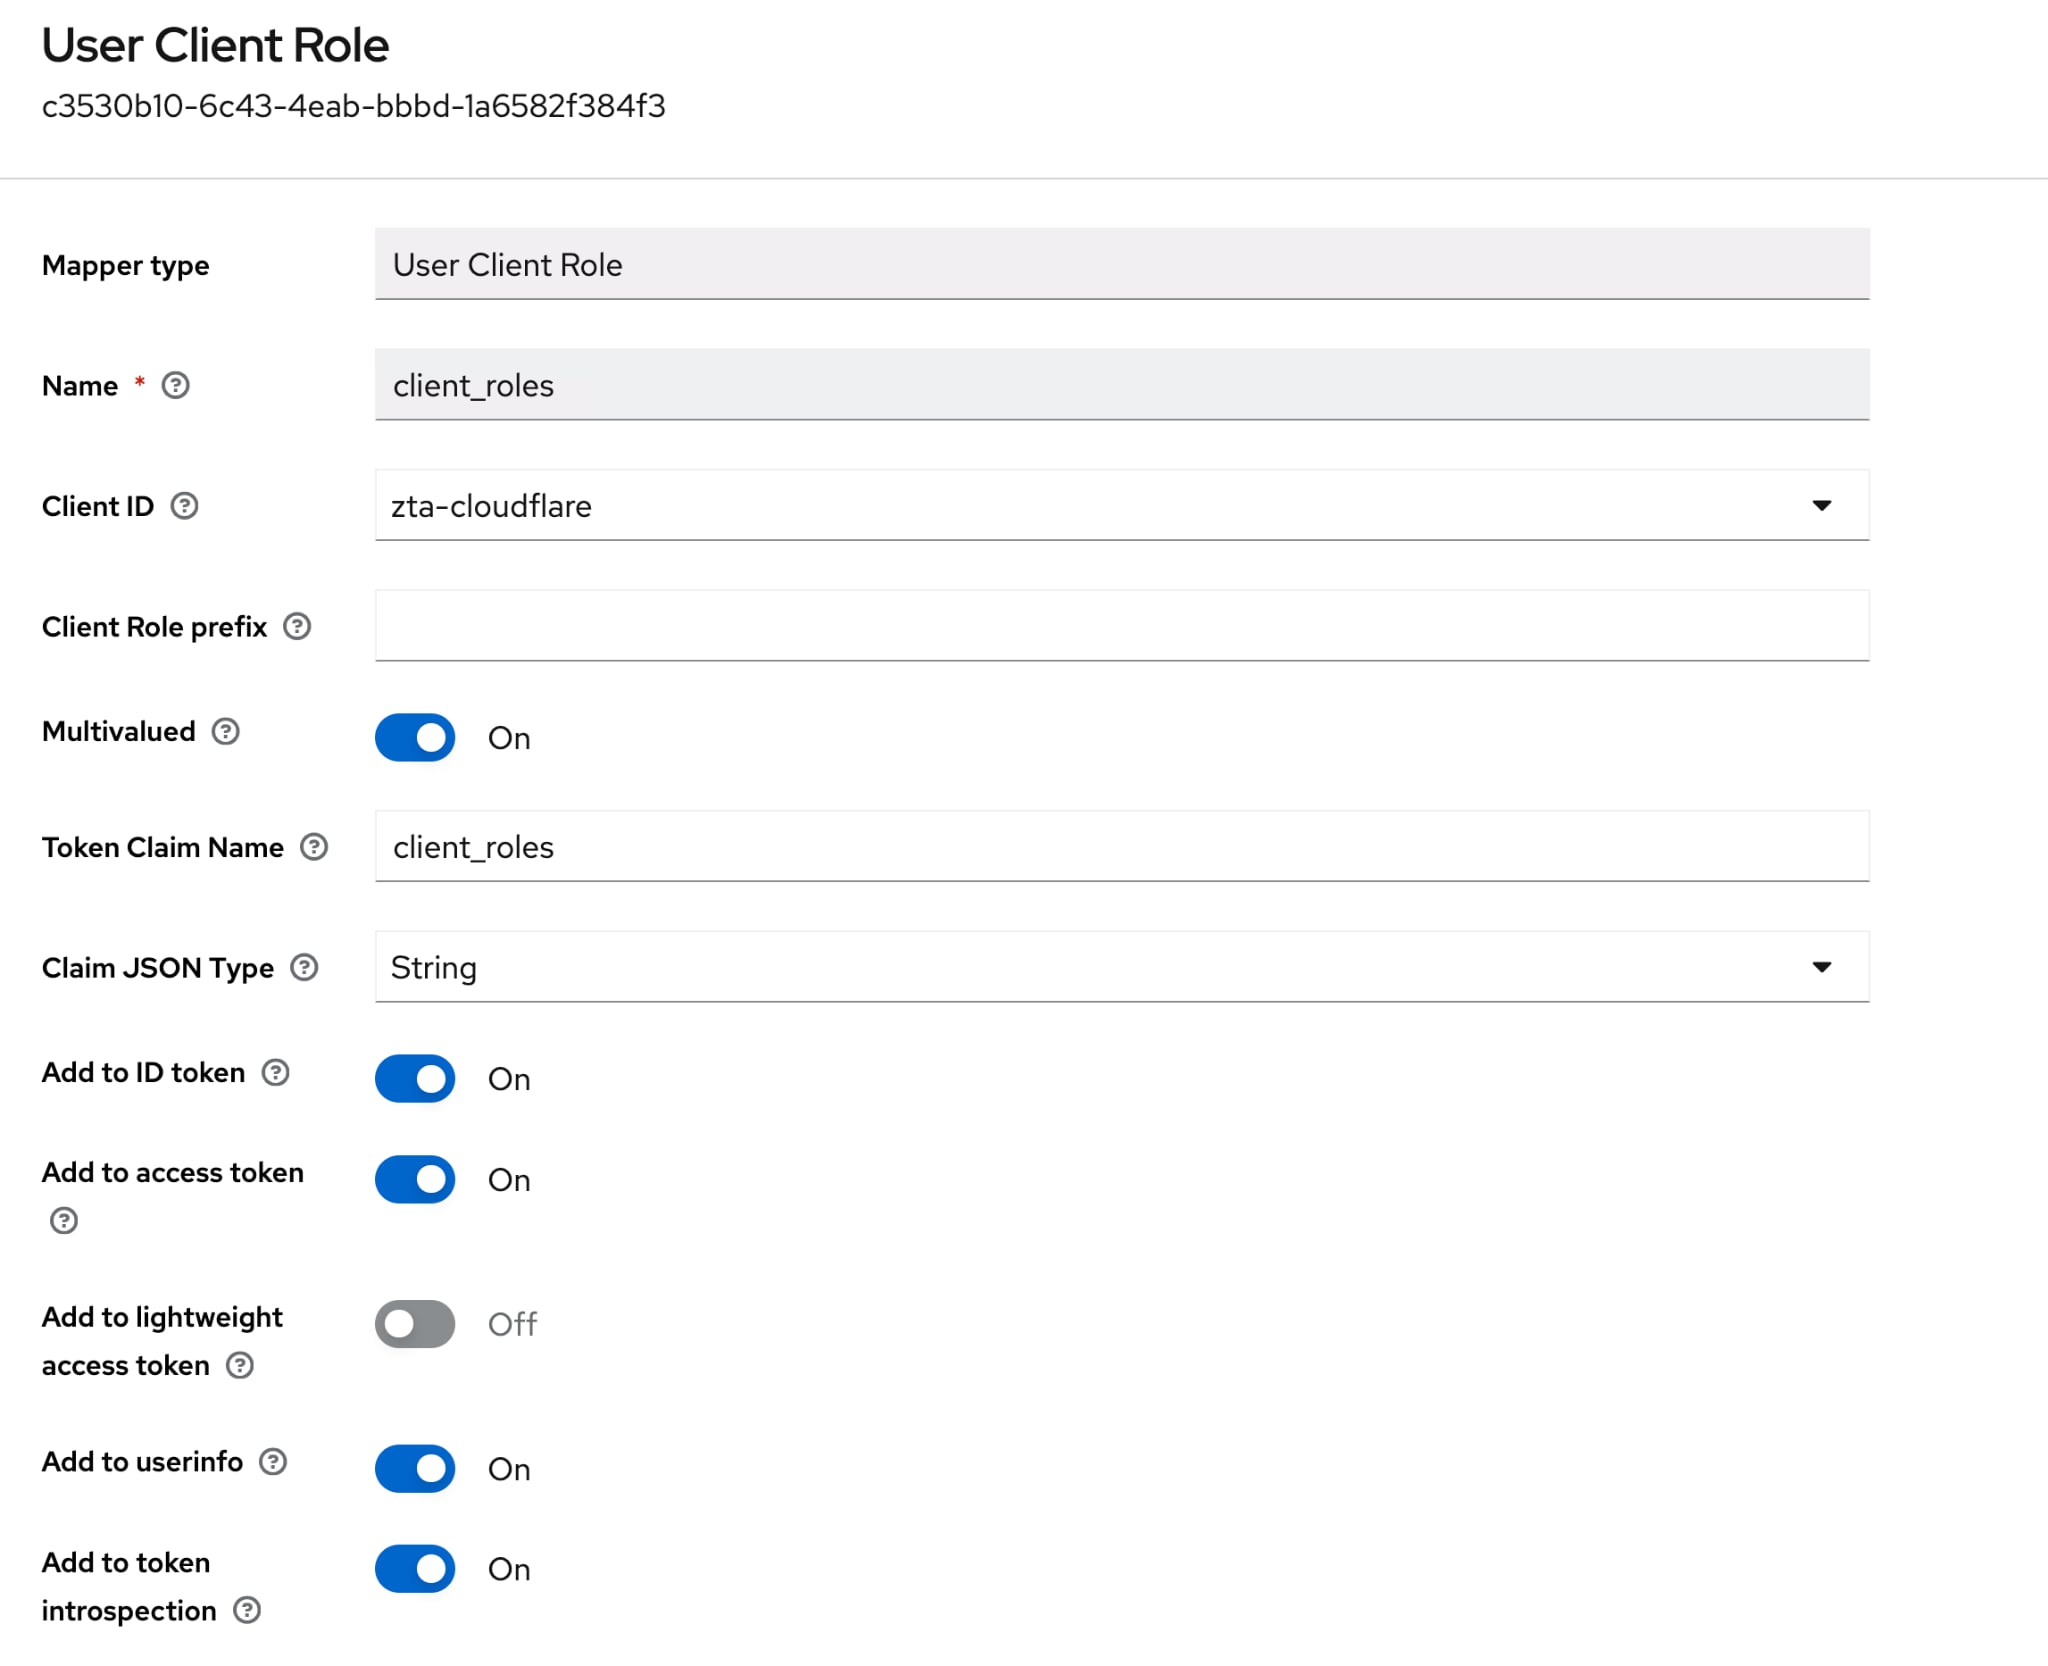
\includegraphics[width=0.5\textwidth]{contents/contents/image_7.png}    
    \caption{Mapper cho Client Role}
    \label{fig:example_image}
    
\end{figure}
 
\begin{figure}[H]
    \centering
    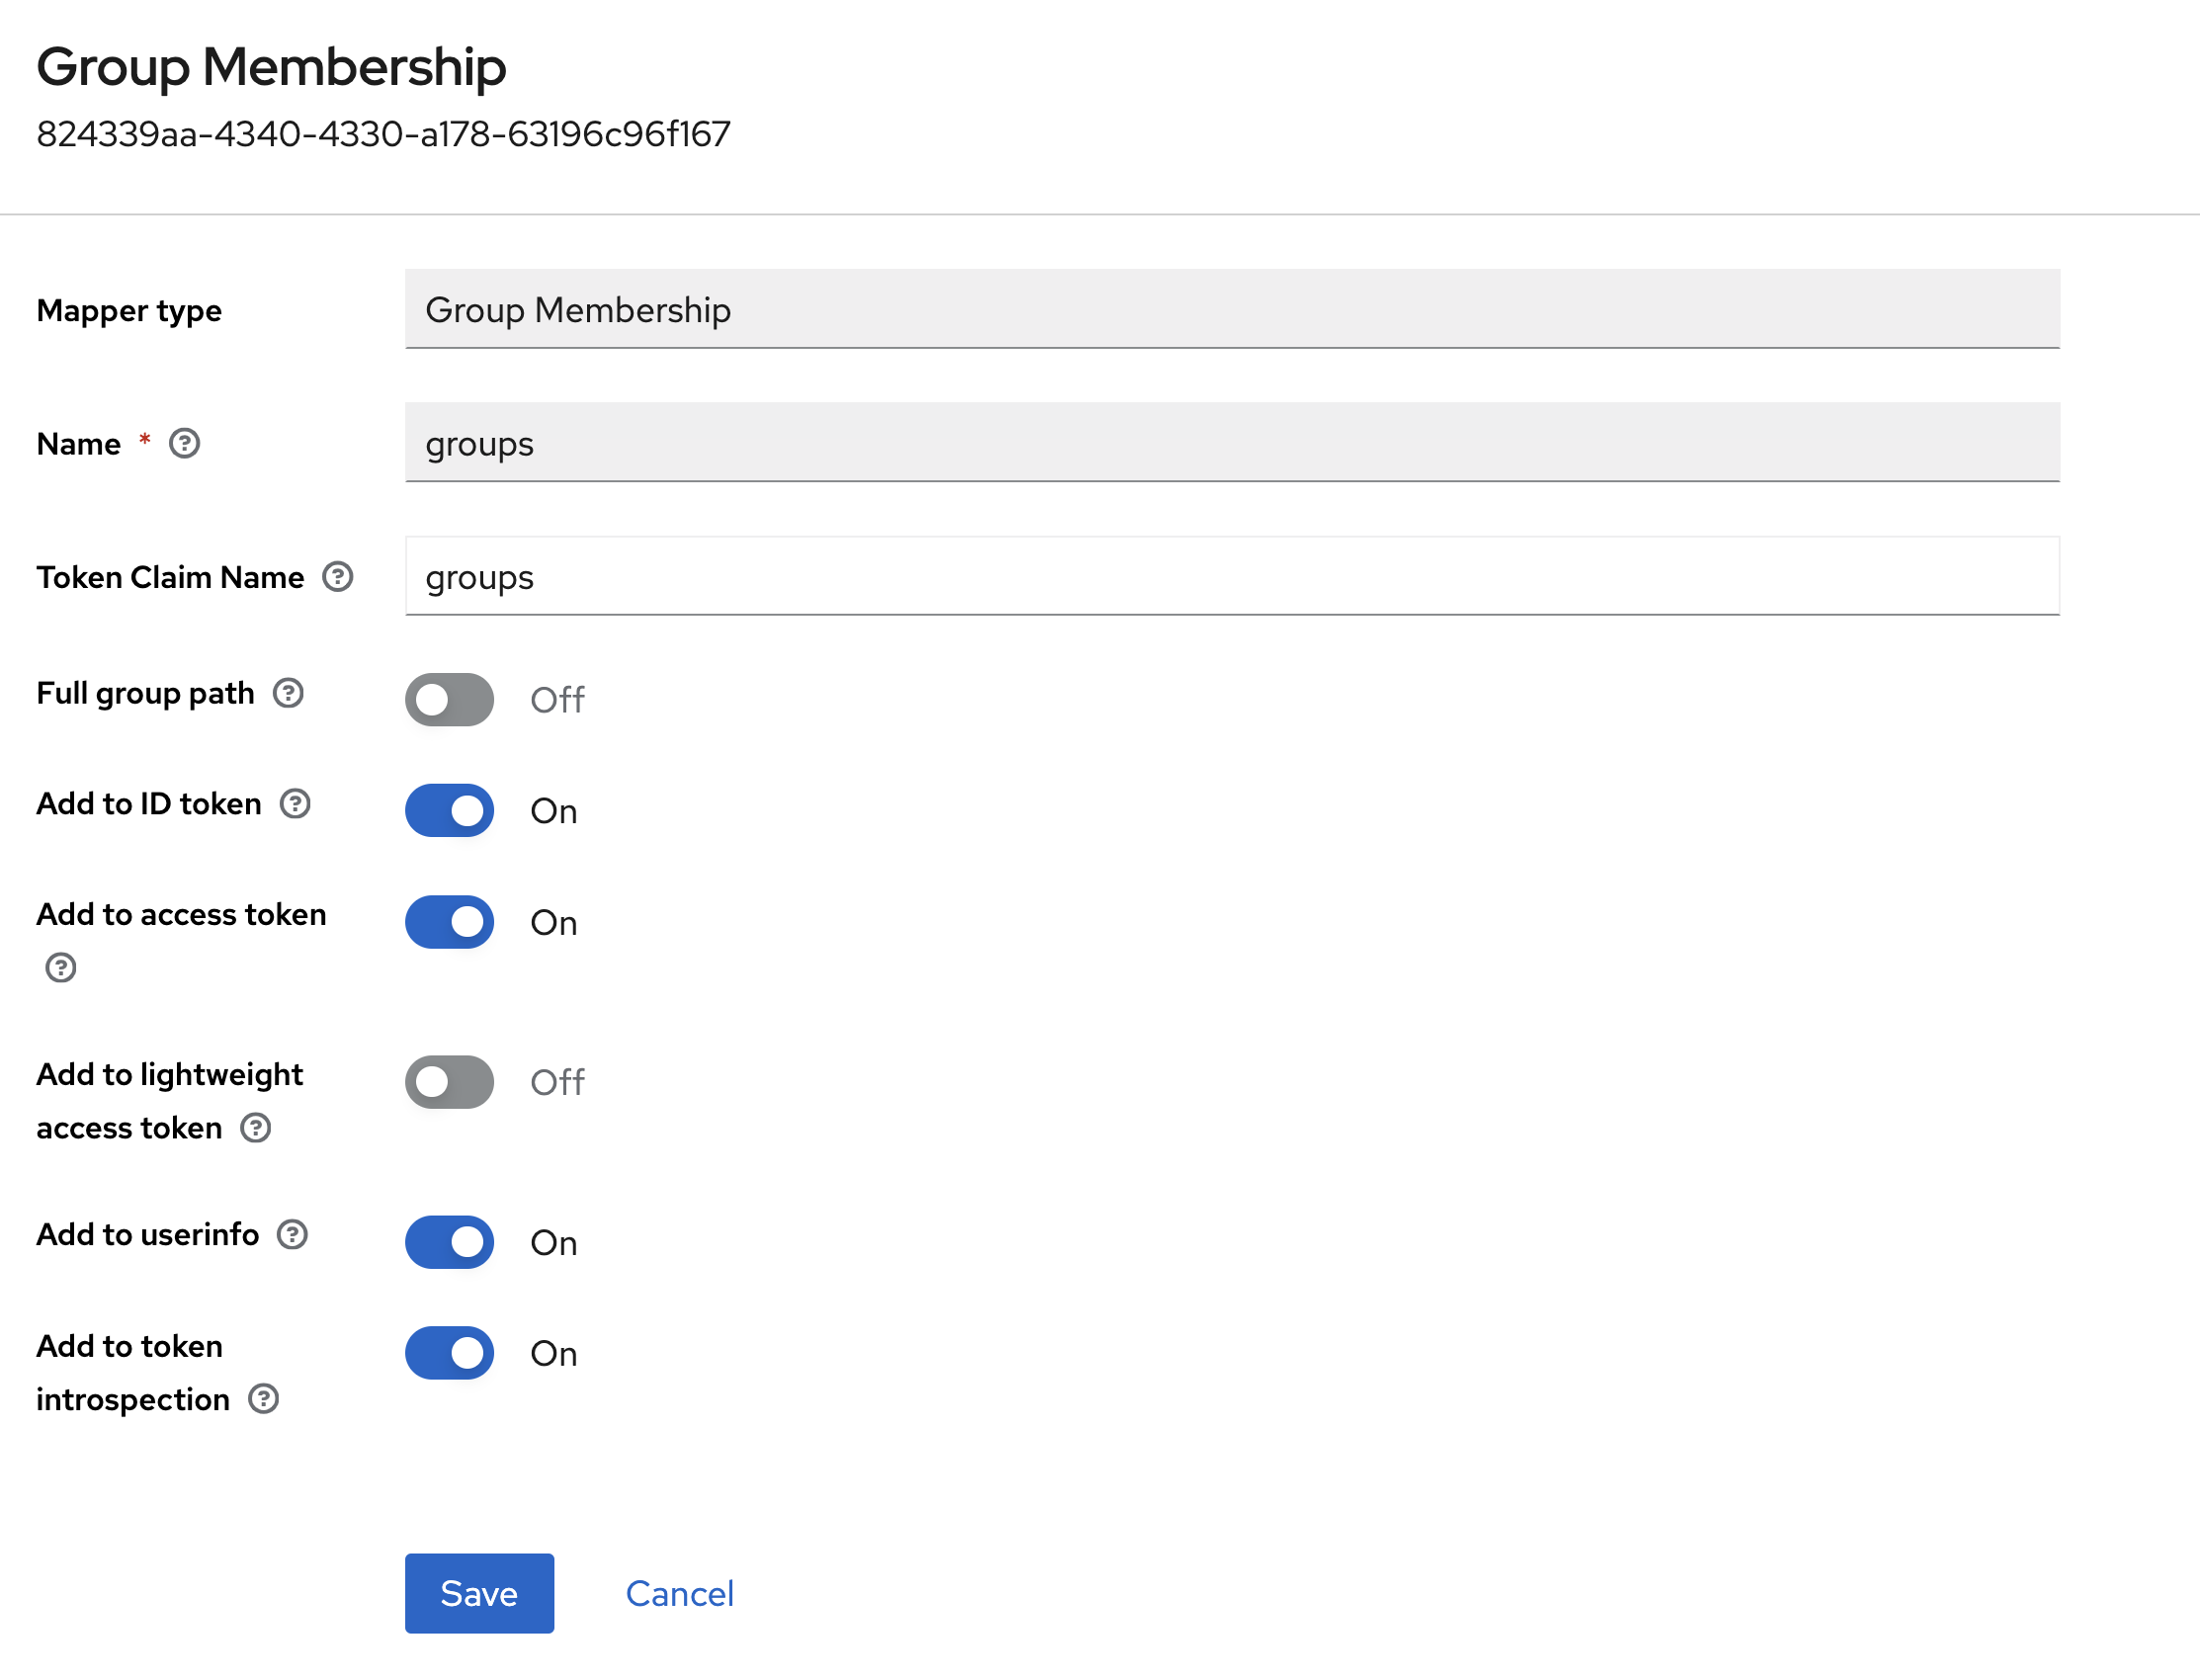
\includegraphics[width=0.5\textwidth]{contents/contents/image_9.png}
    \caption{Mapper cho Group Membership}
    \label{fig:example_image}
    
\end{figure}

Các nội dung dùng để xác minh danh tính được claims thông qua các mapper được tạo bên trên lấy tên, token claim name và loại dữ liệu phù hợp tương ứng. Ví dụ tên groups, token claimname là group và mapper type là group membership 
\begin{figure}[H]
    \centering
    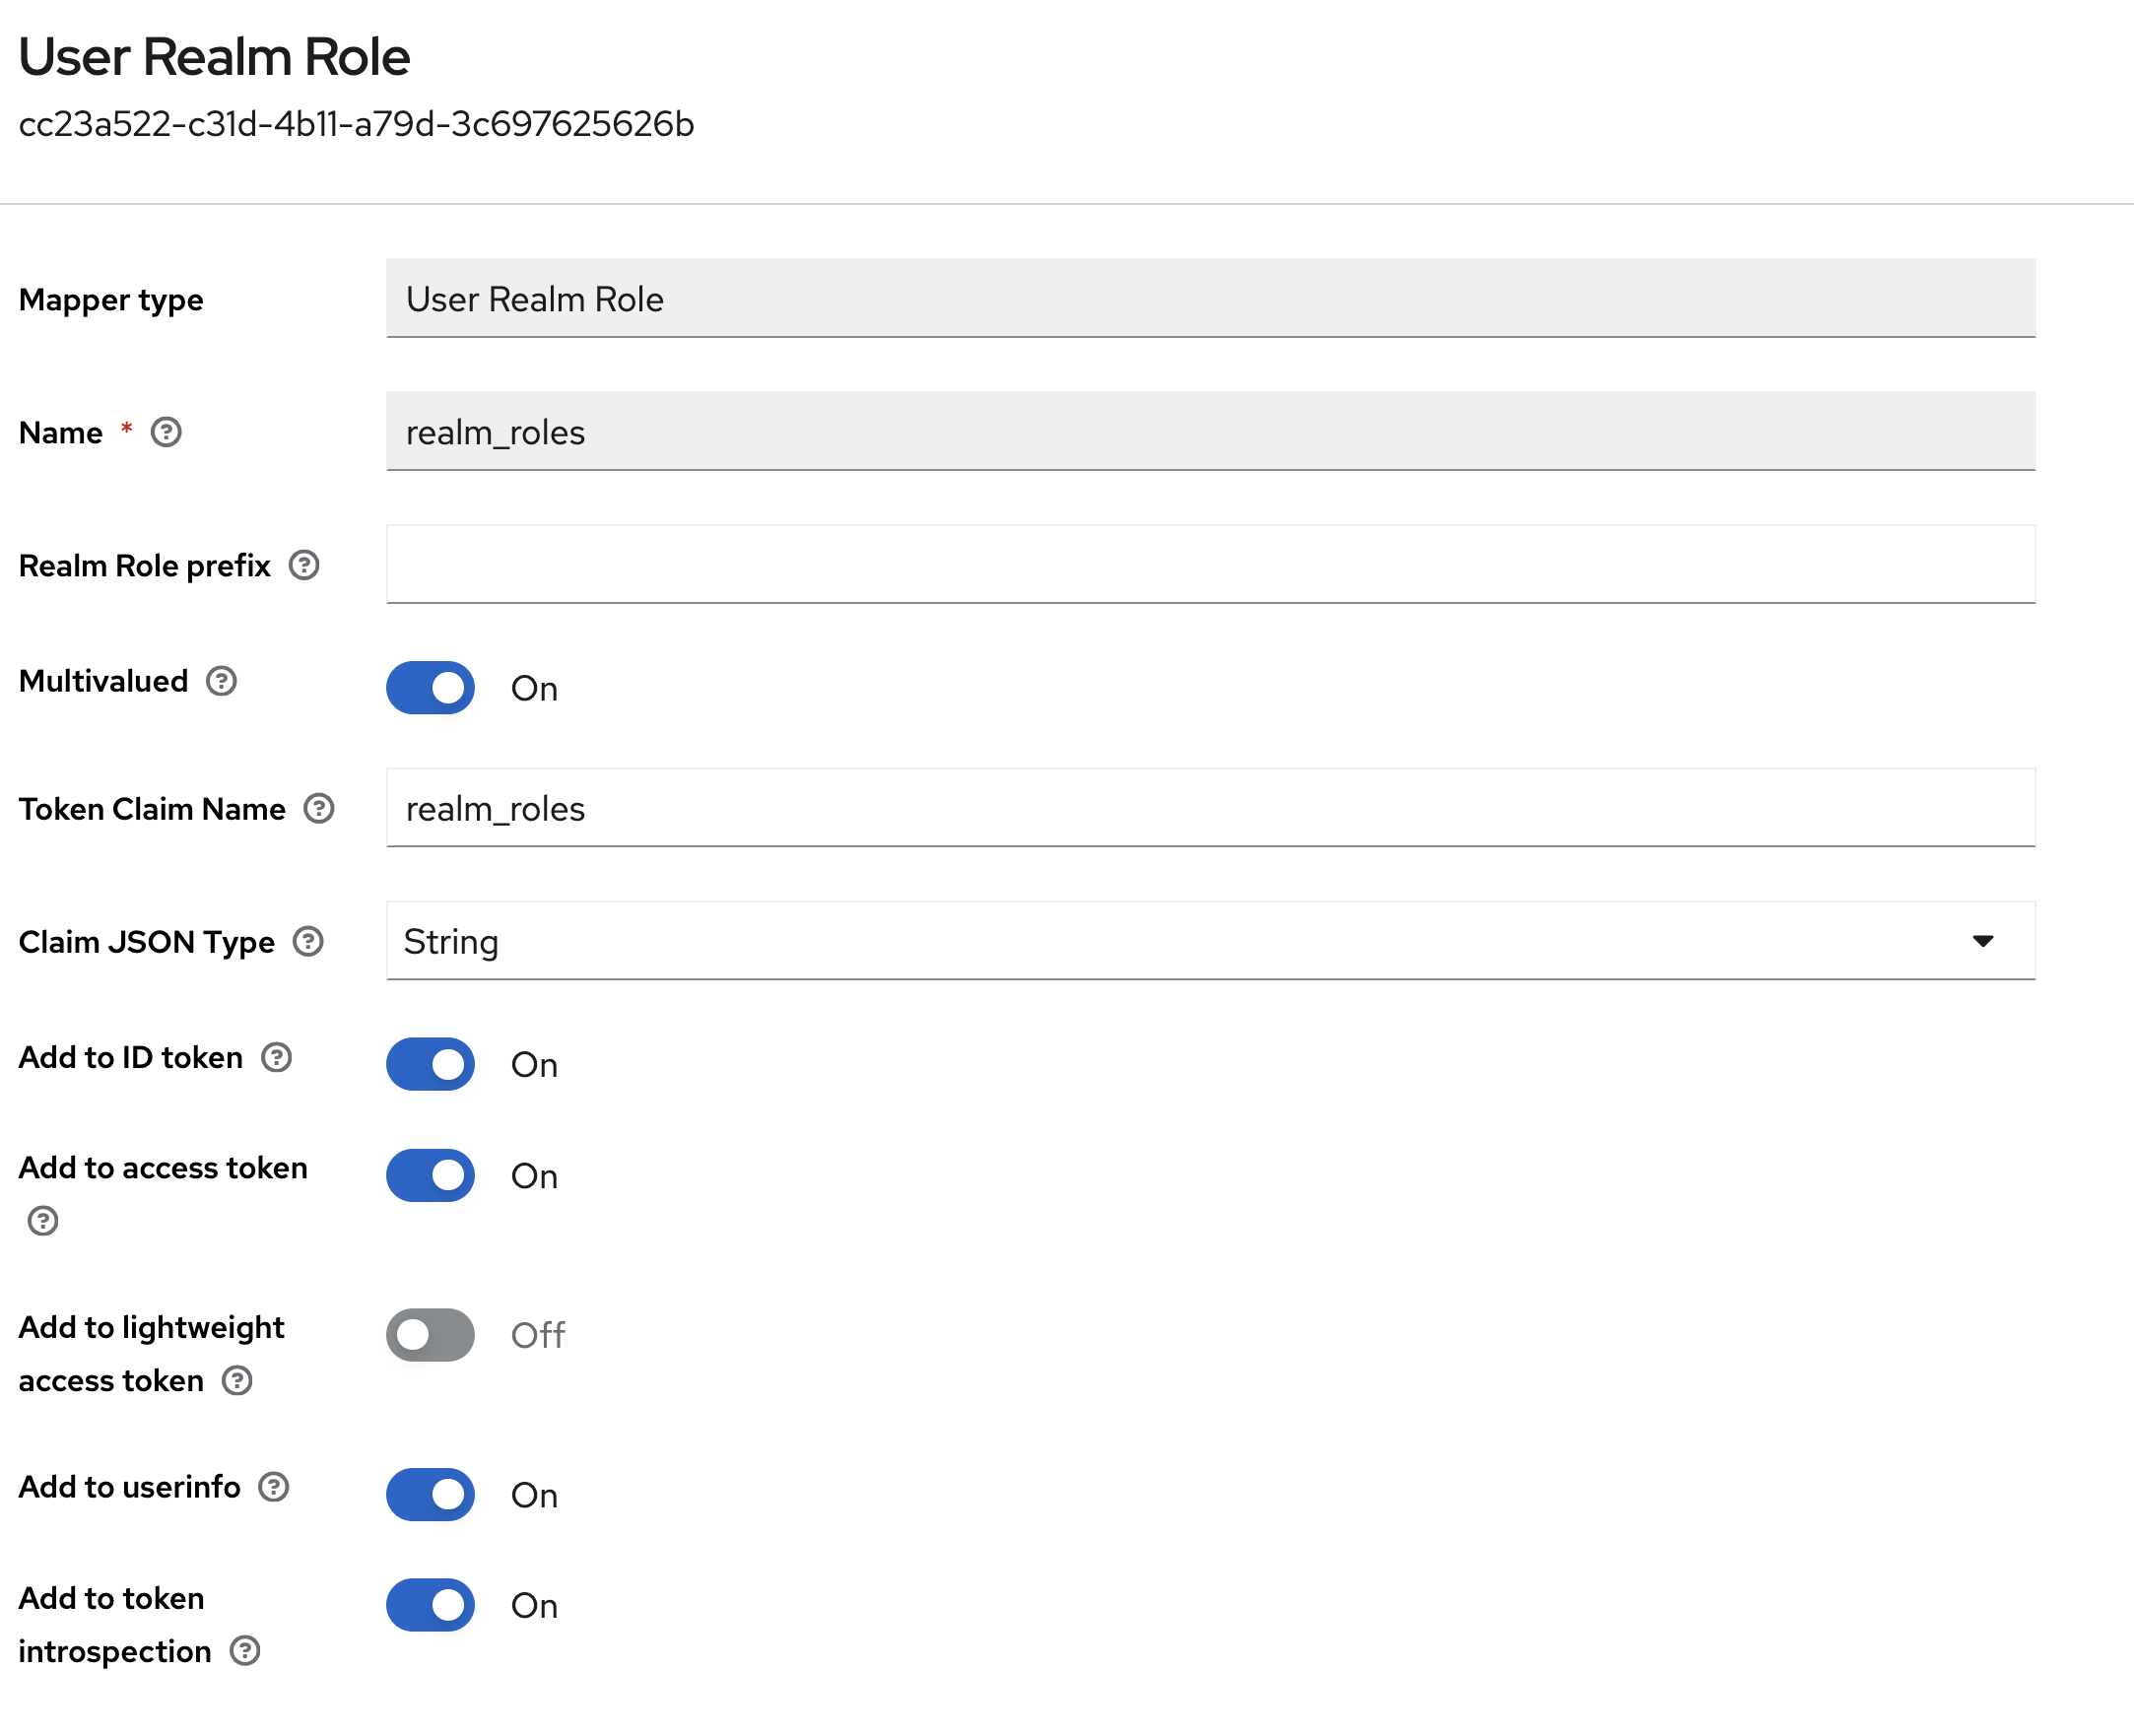
\includegraphics[width=0.5\textwidth]{contents/contents/image_10.png}
    \caption{Mapper cho User Realm Role}
    \label{fig:example_image}
    
\end{figure}

\begin{figure}[H]
    \centering
    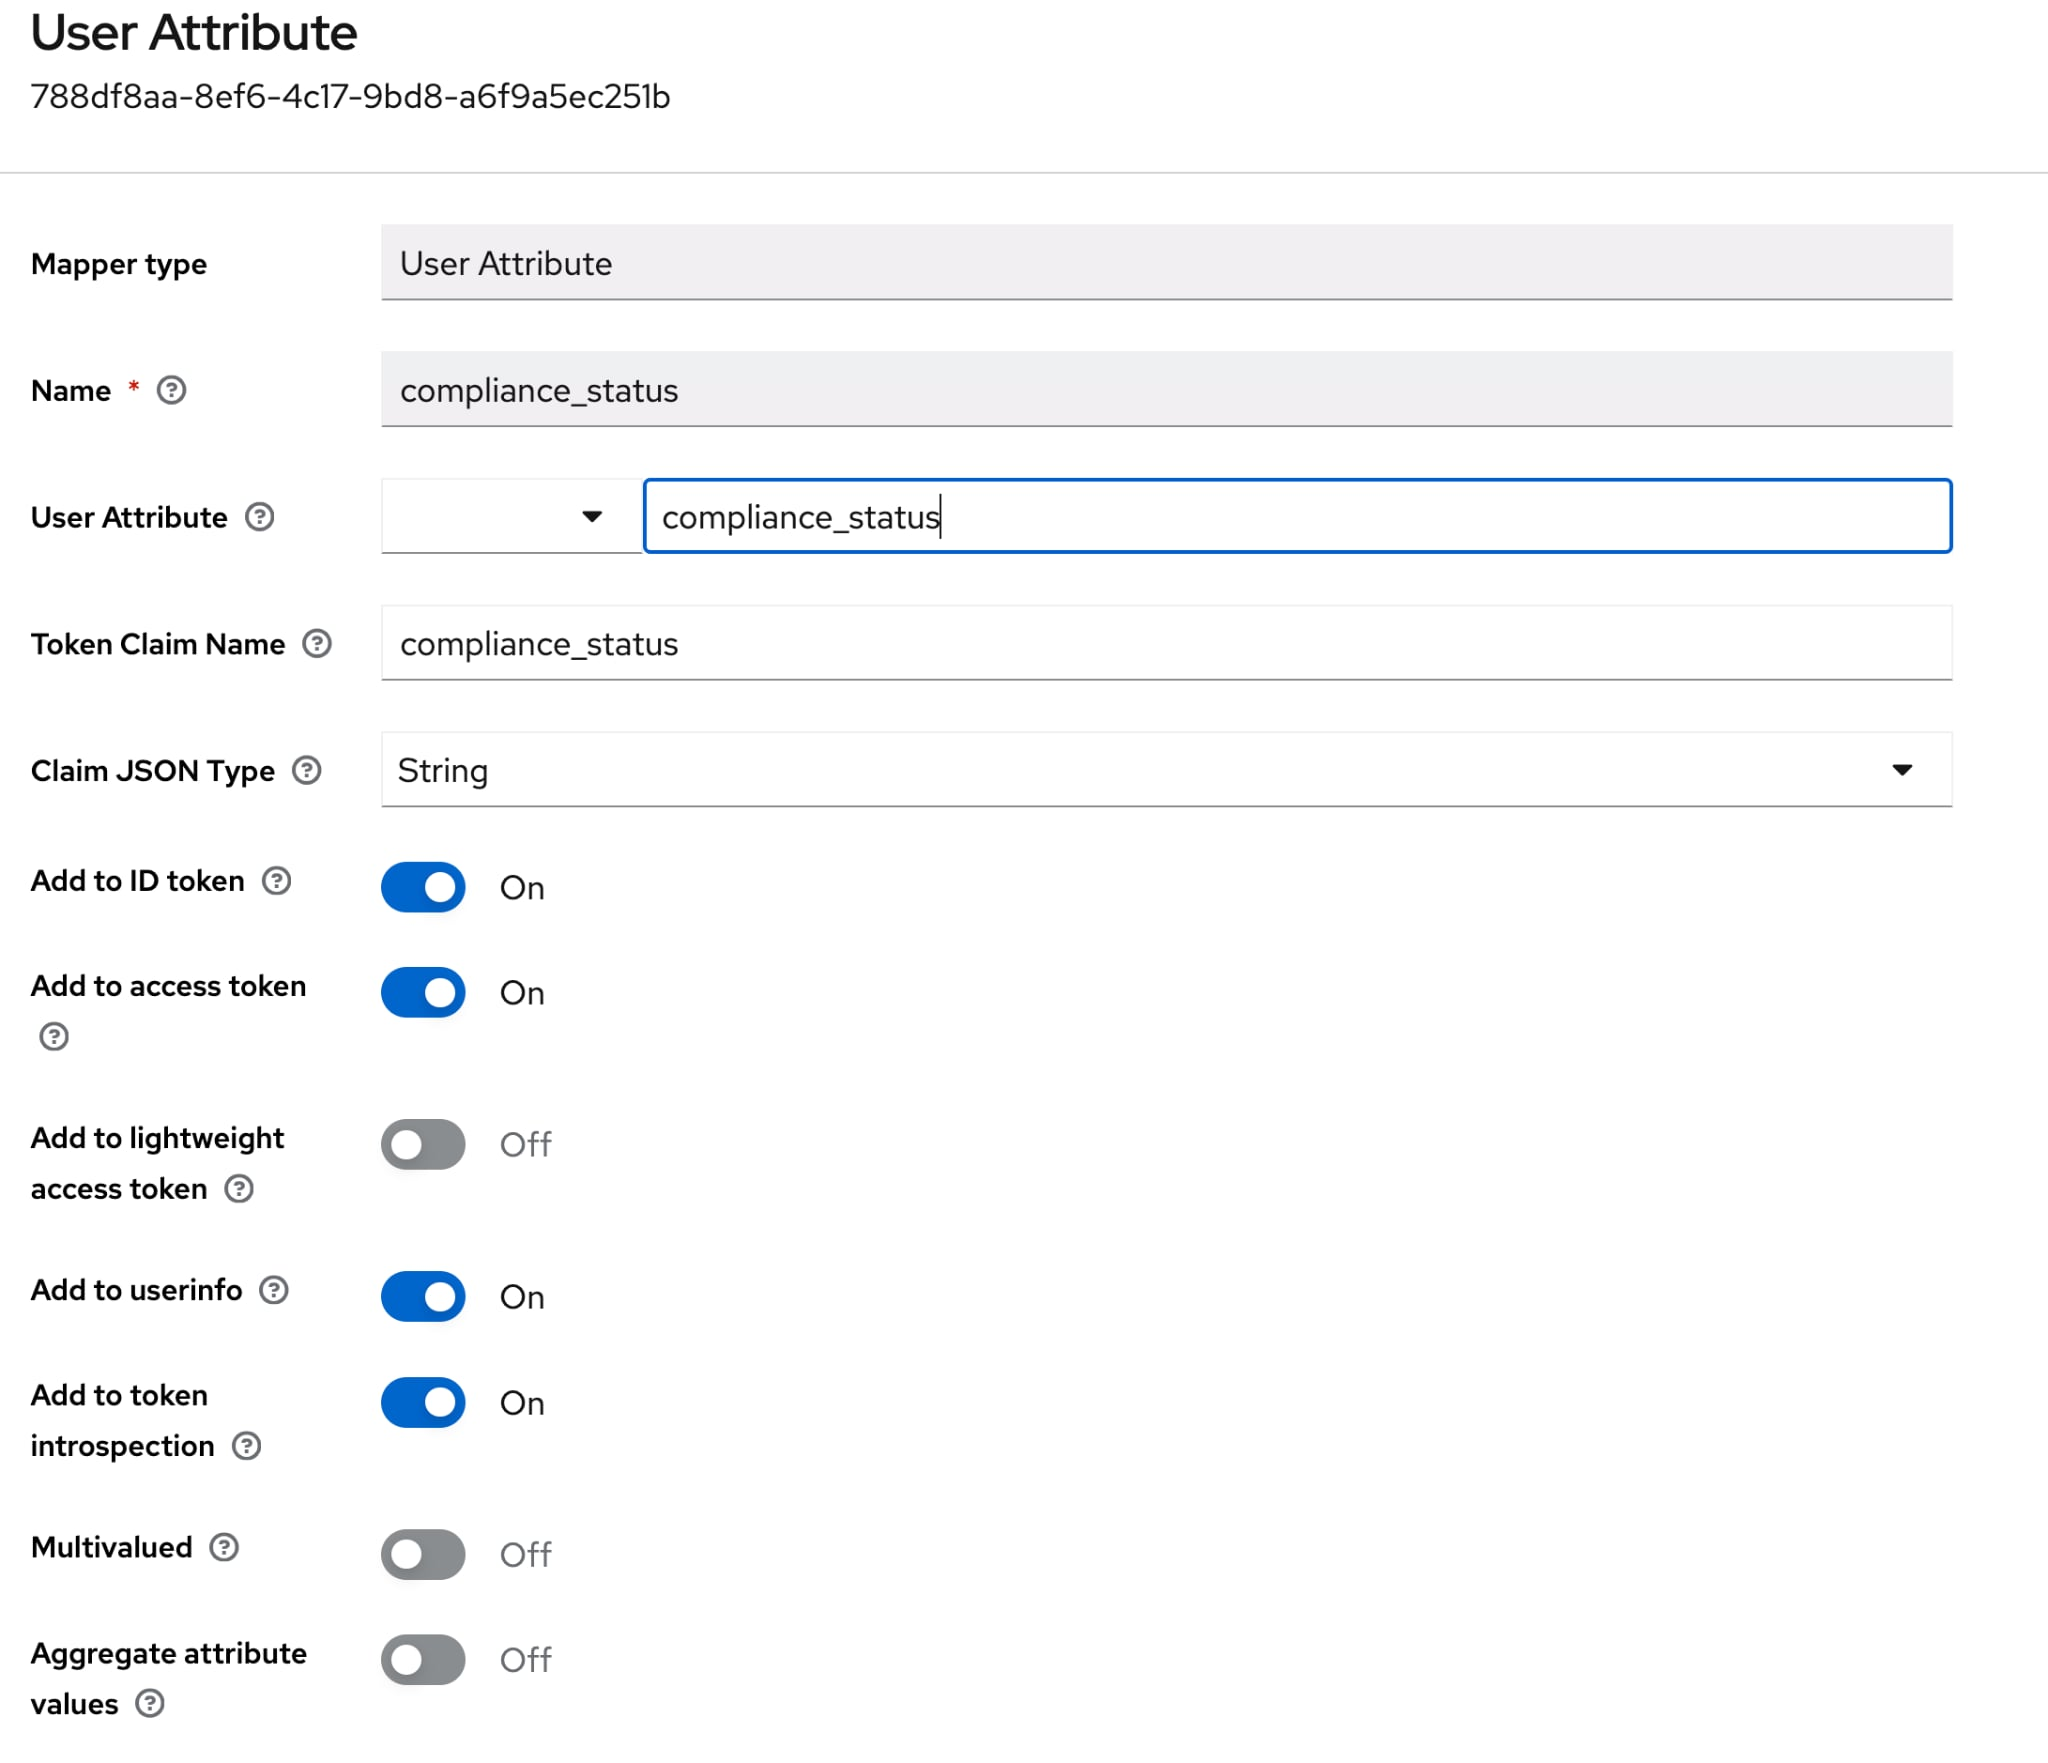
\includegraphics[width=0.5\textwidth]{contents/contents/image_8.png}
    \caption{Các Mapper cho User Attribute}
    \label{fig:example_image}
    
\end{figure}

\begin{figure}[H]
    \centering
    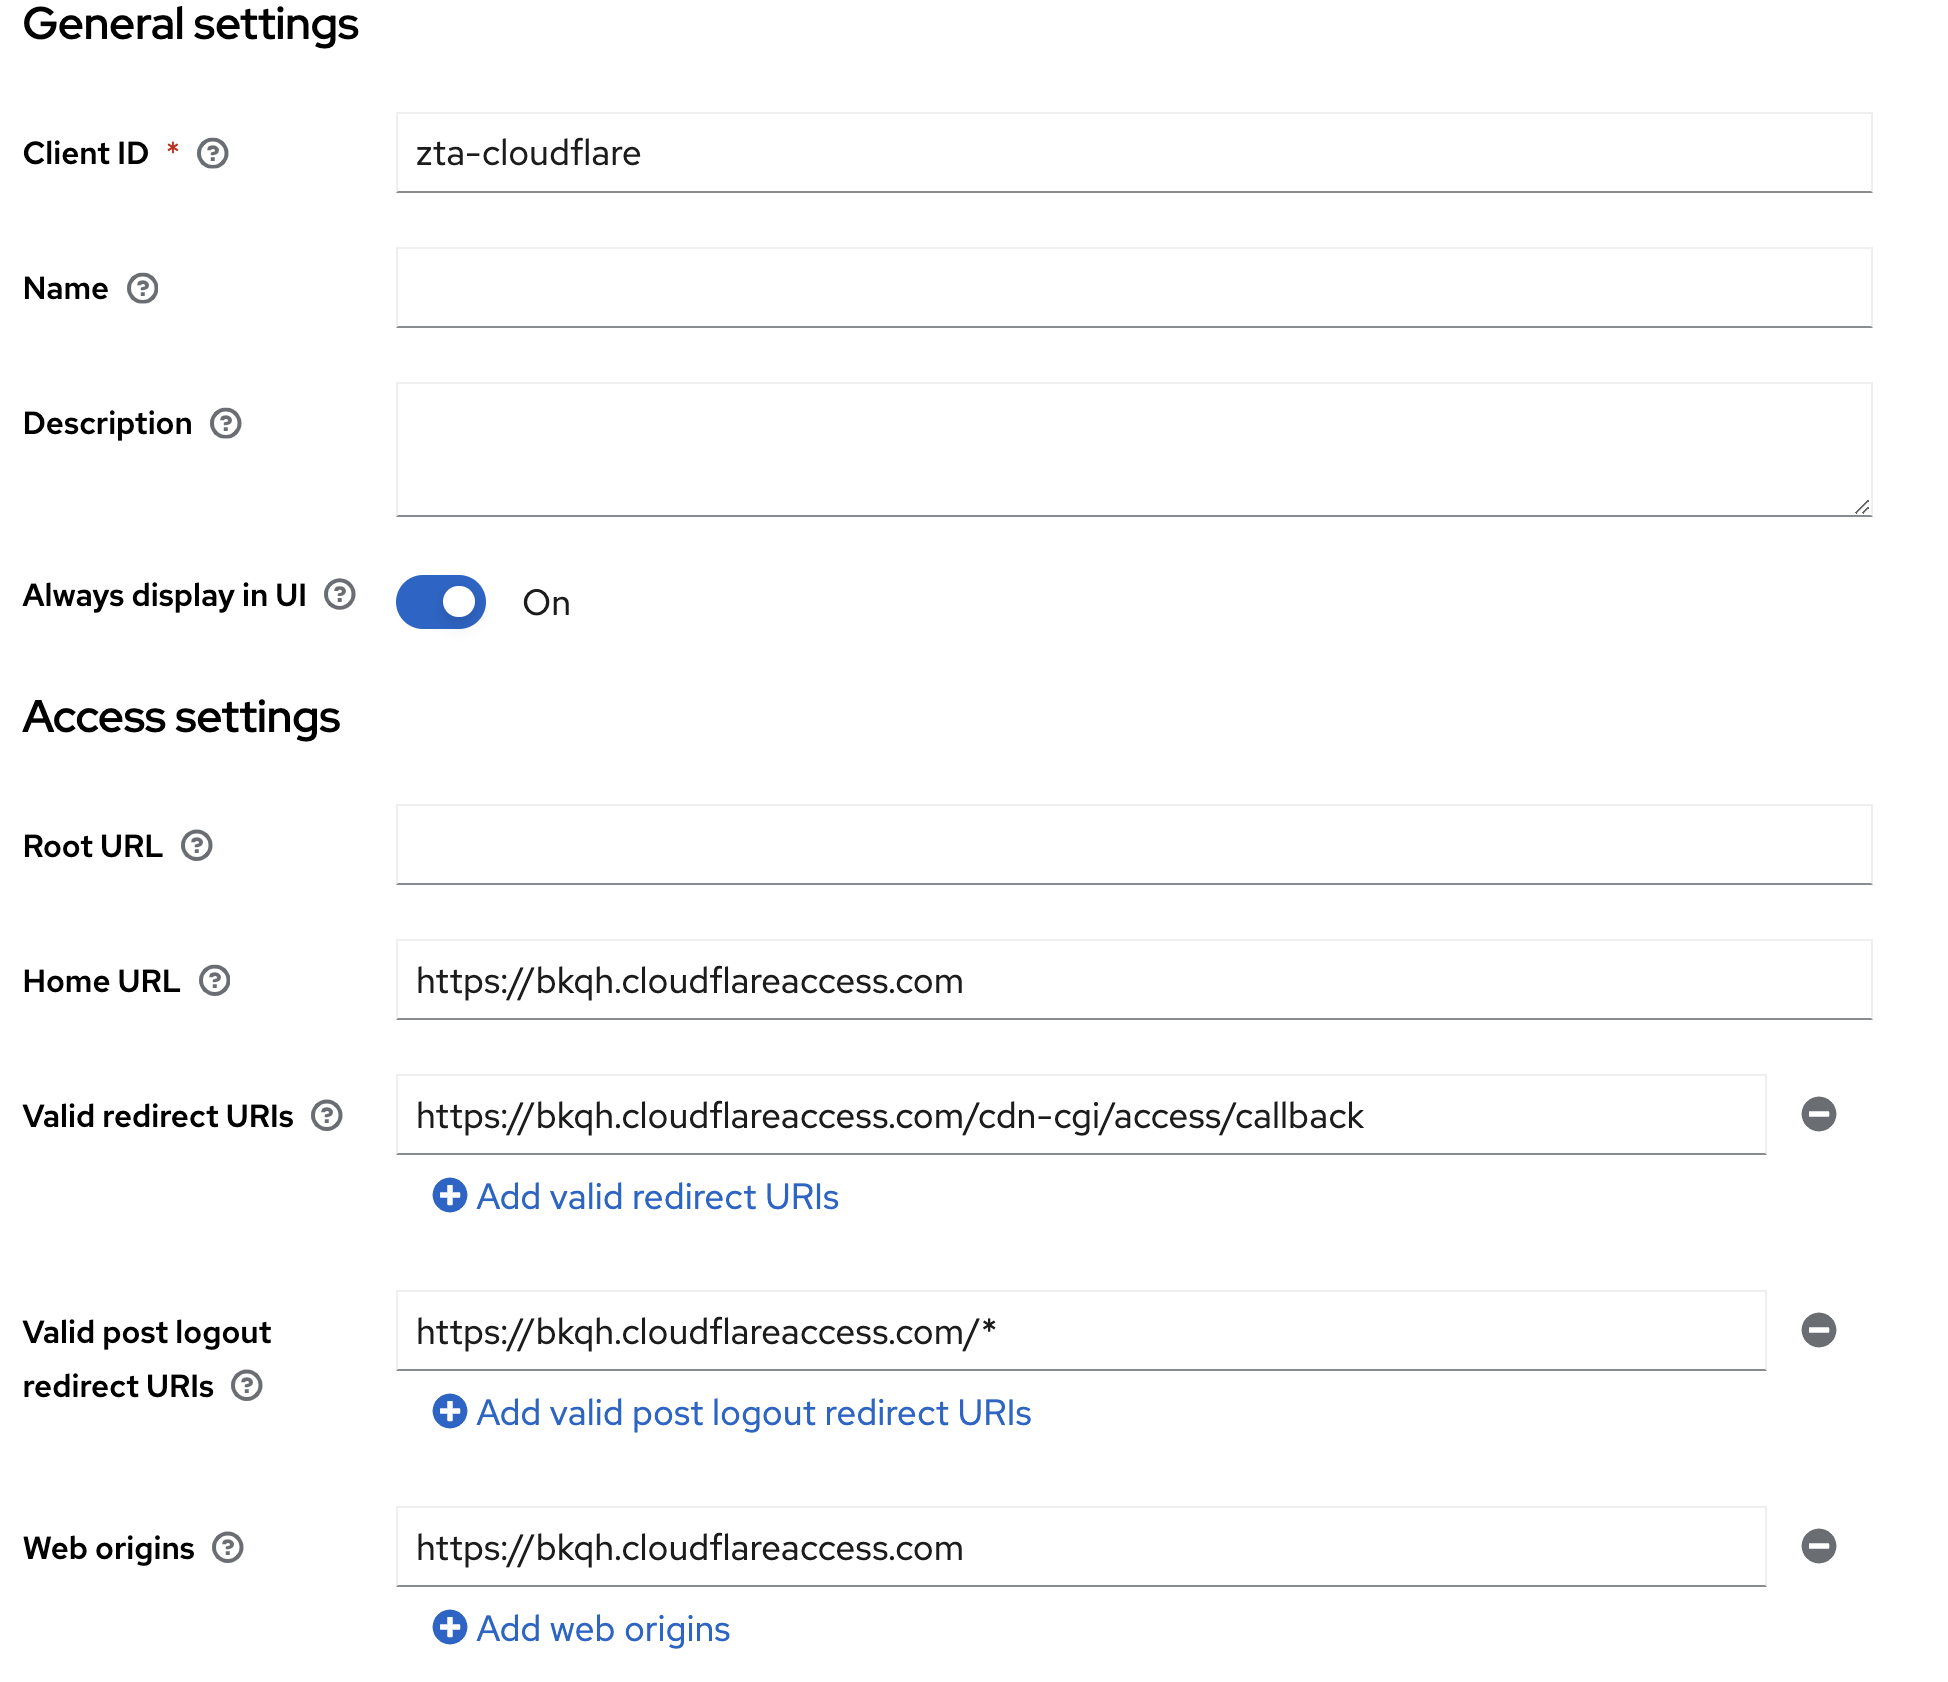
\includegraphics[width=0.8\textwidth]{contents/contents/image_2.png}
    \caption{Cấu hình cho Keycloak Client}
    \label{fig:example_image}
    
\end{figure}
\begin{figure}[H]
    \centering
    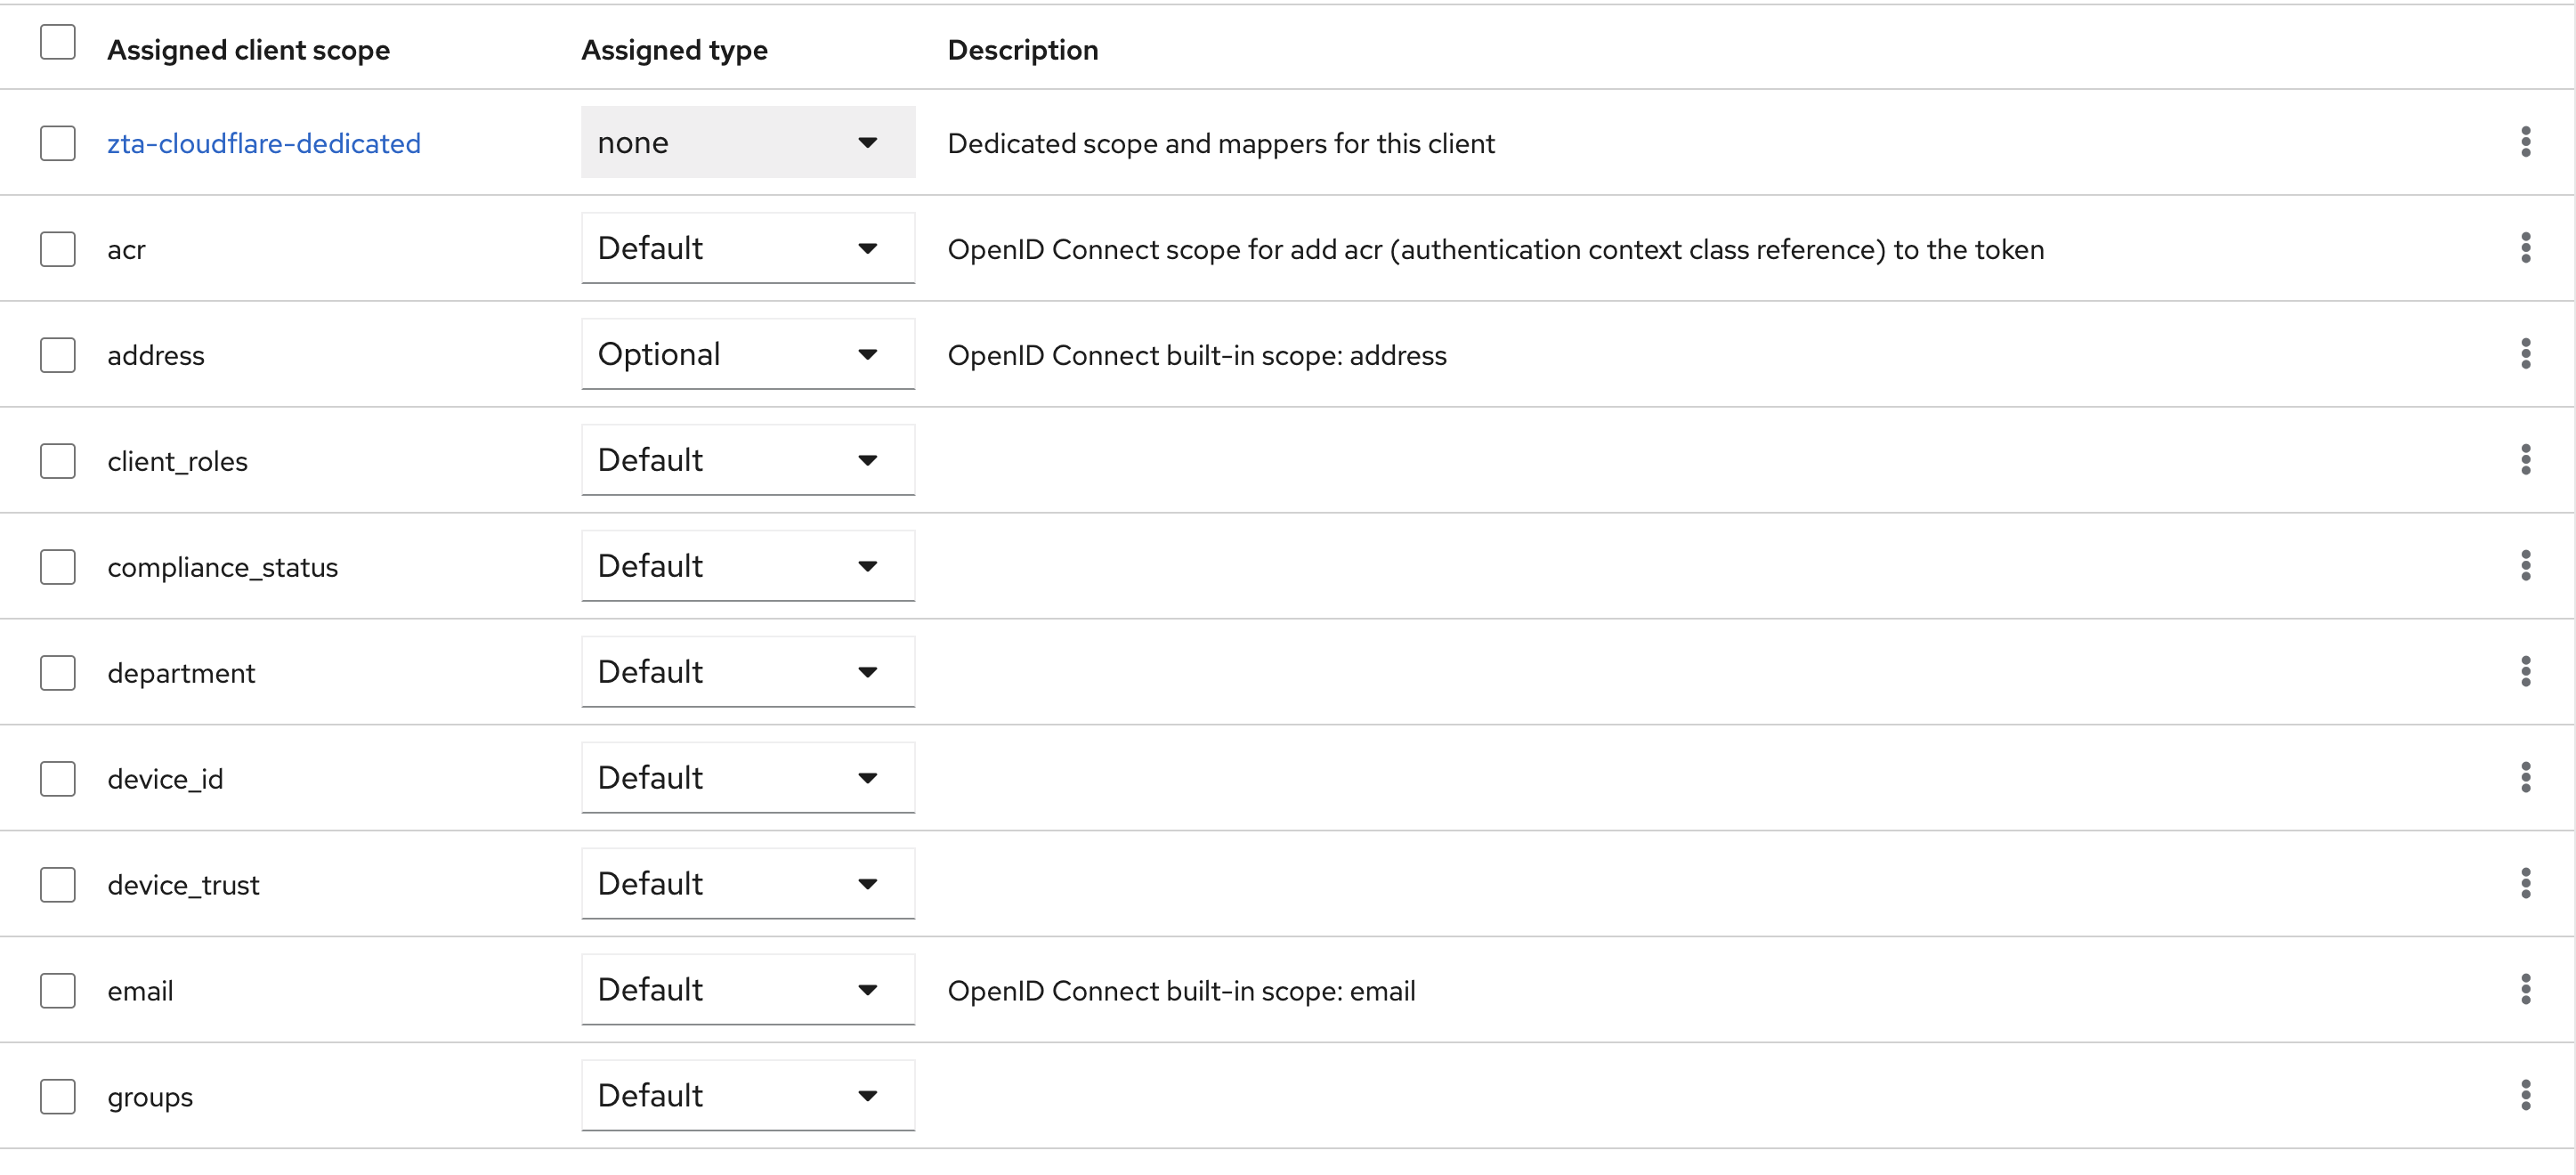
\includegraphics[width=0.5\textwidth]{contents/contents/image_3.png}    
    \caption{Cấu hình client scope}
    \label{fig:example_image}
    
\end{figure}

\begin{figure}[H]
    \centering
    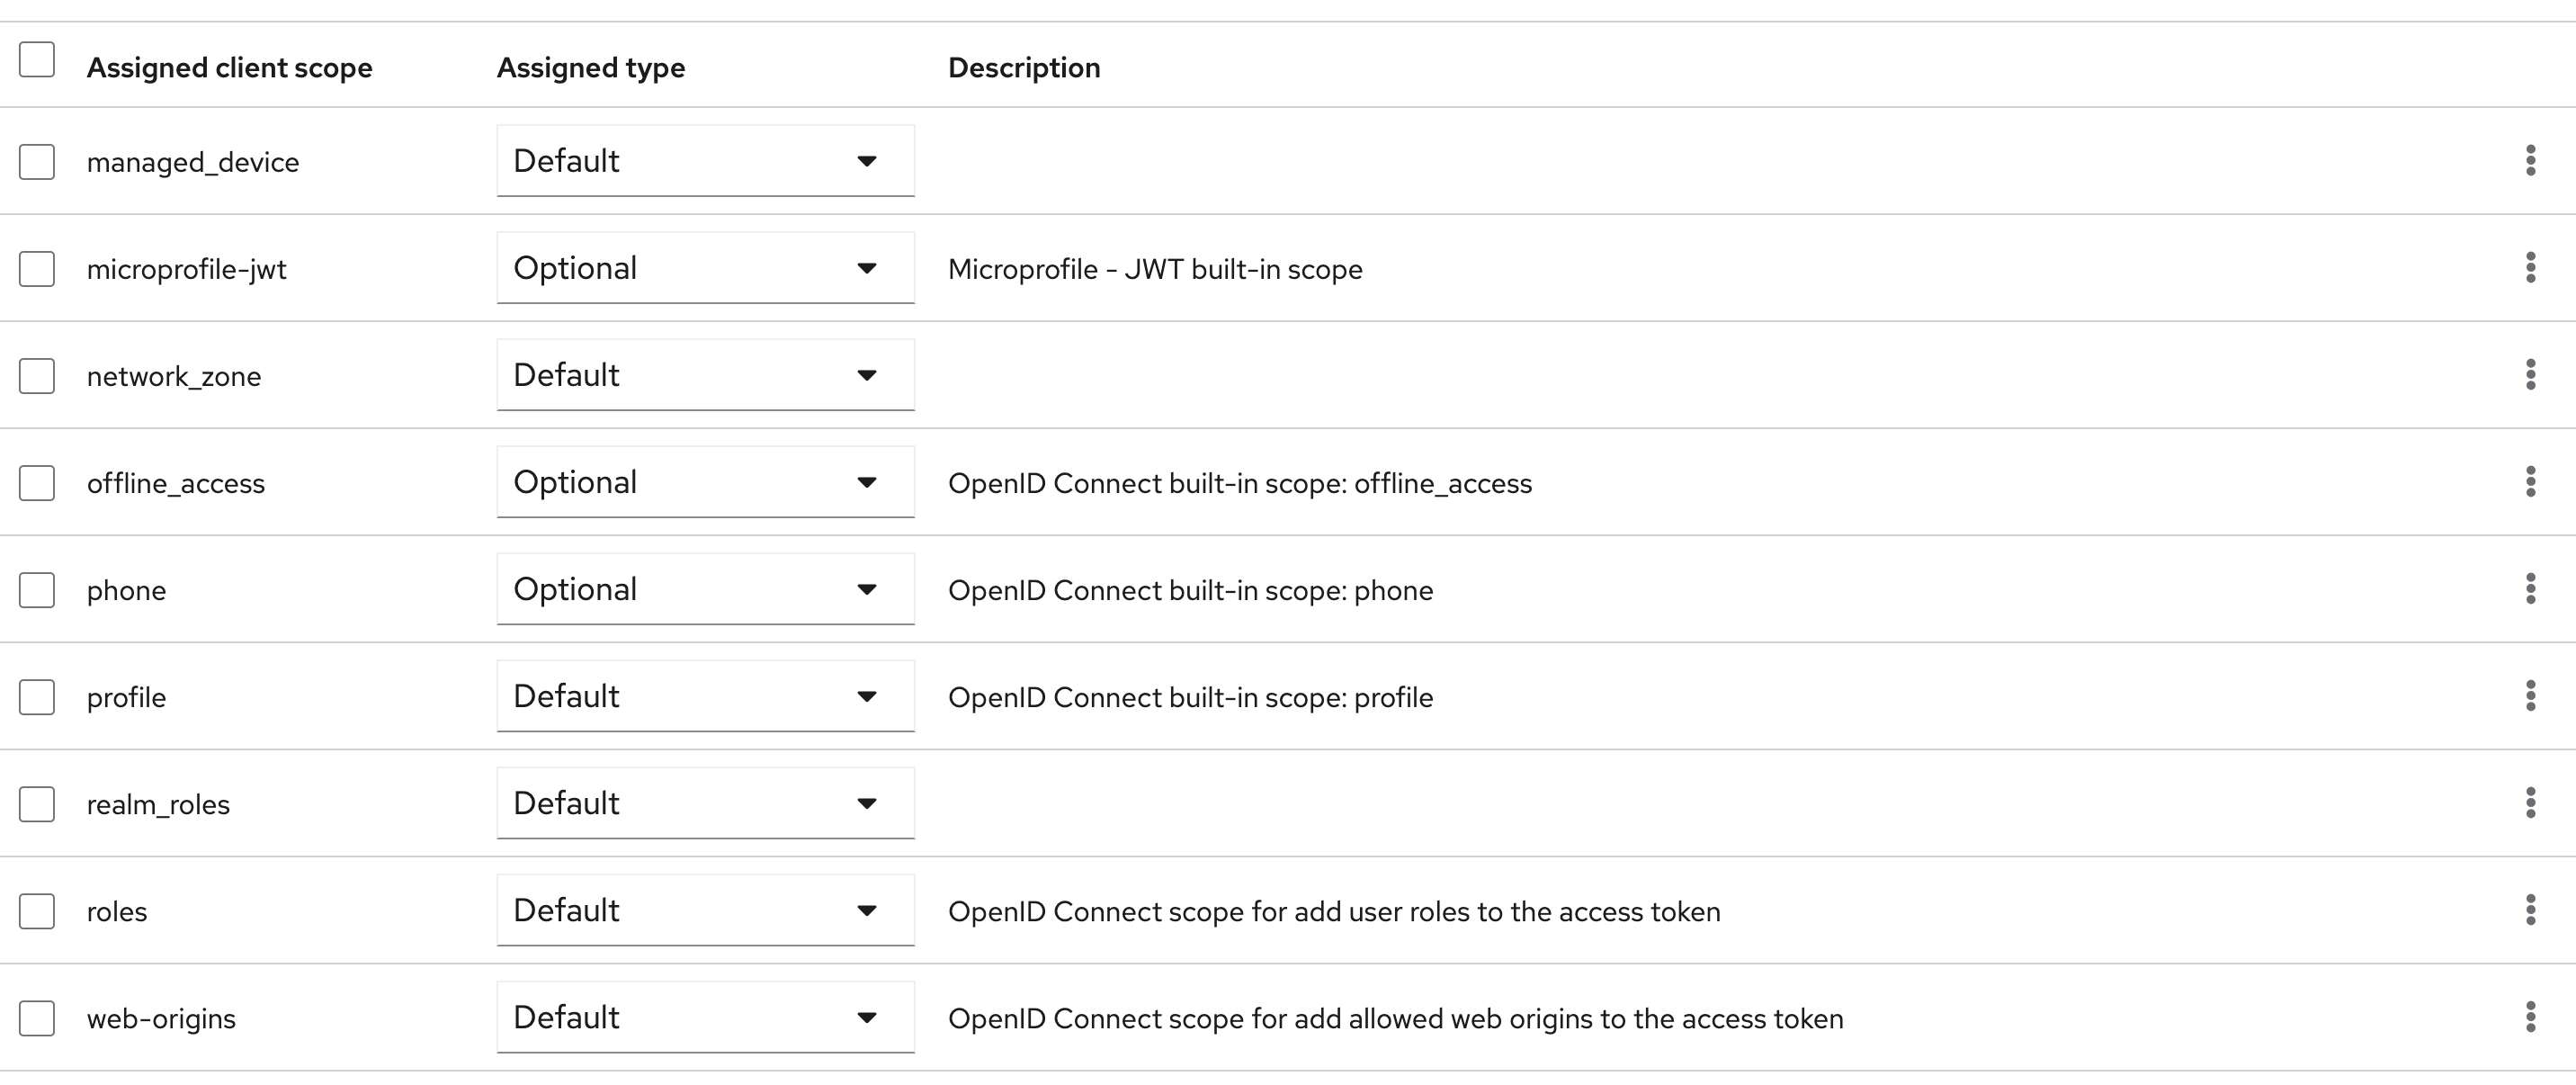
\includegraphics[width=0.5\textwidth]{contents/contents/image_4.png}    
    \caption{Cấu hình client scope}
    \label{fig:example_image}
    
\end{figure}

\begin{figure}[H]
    \centering
    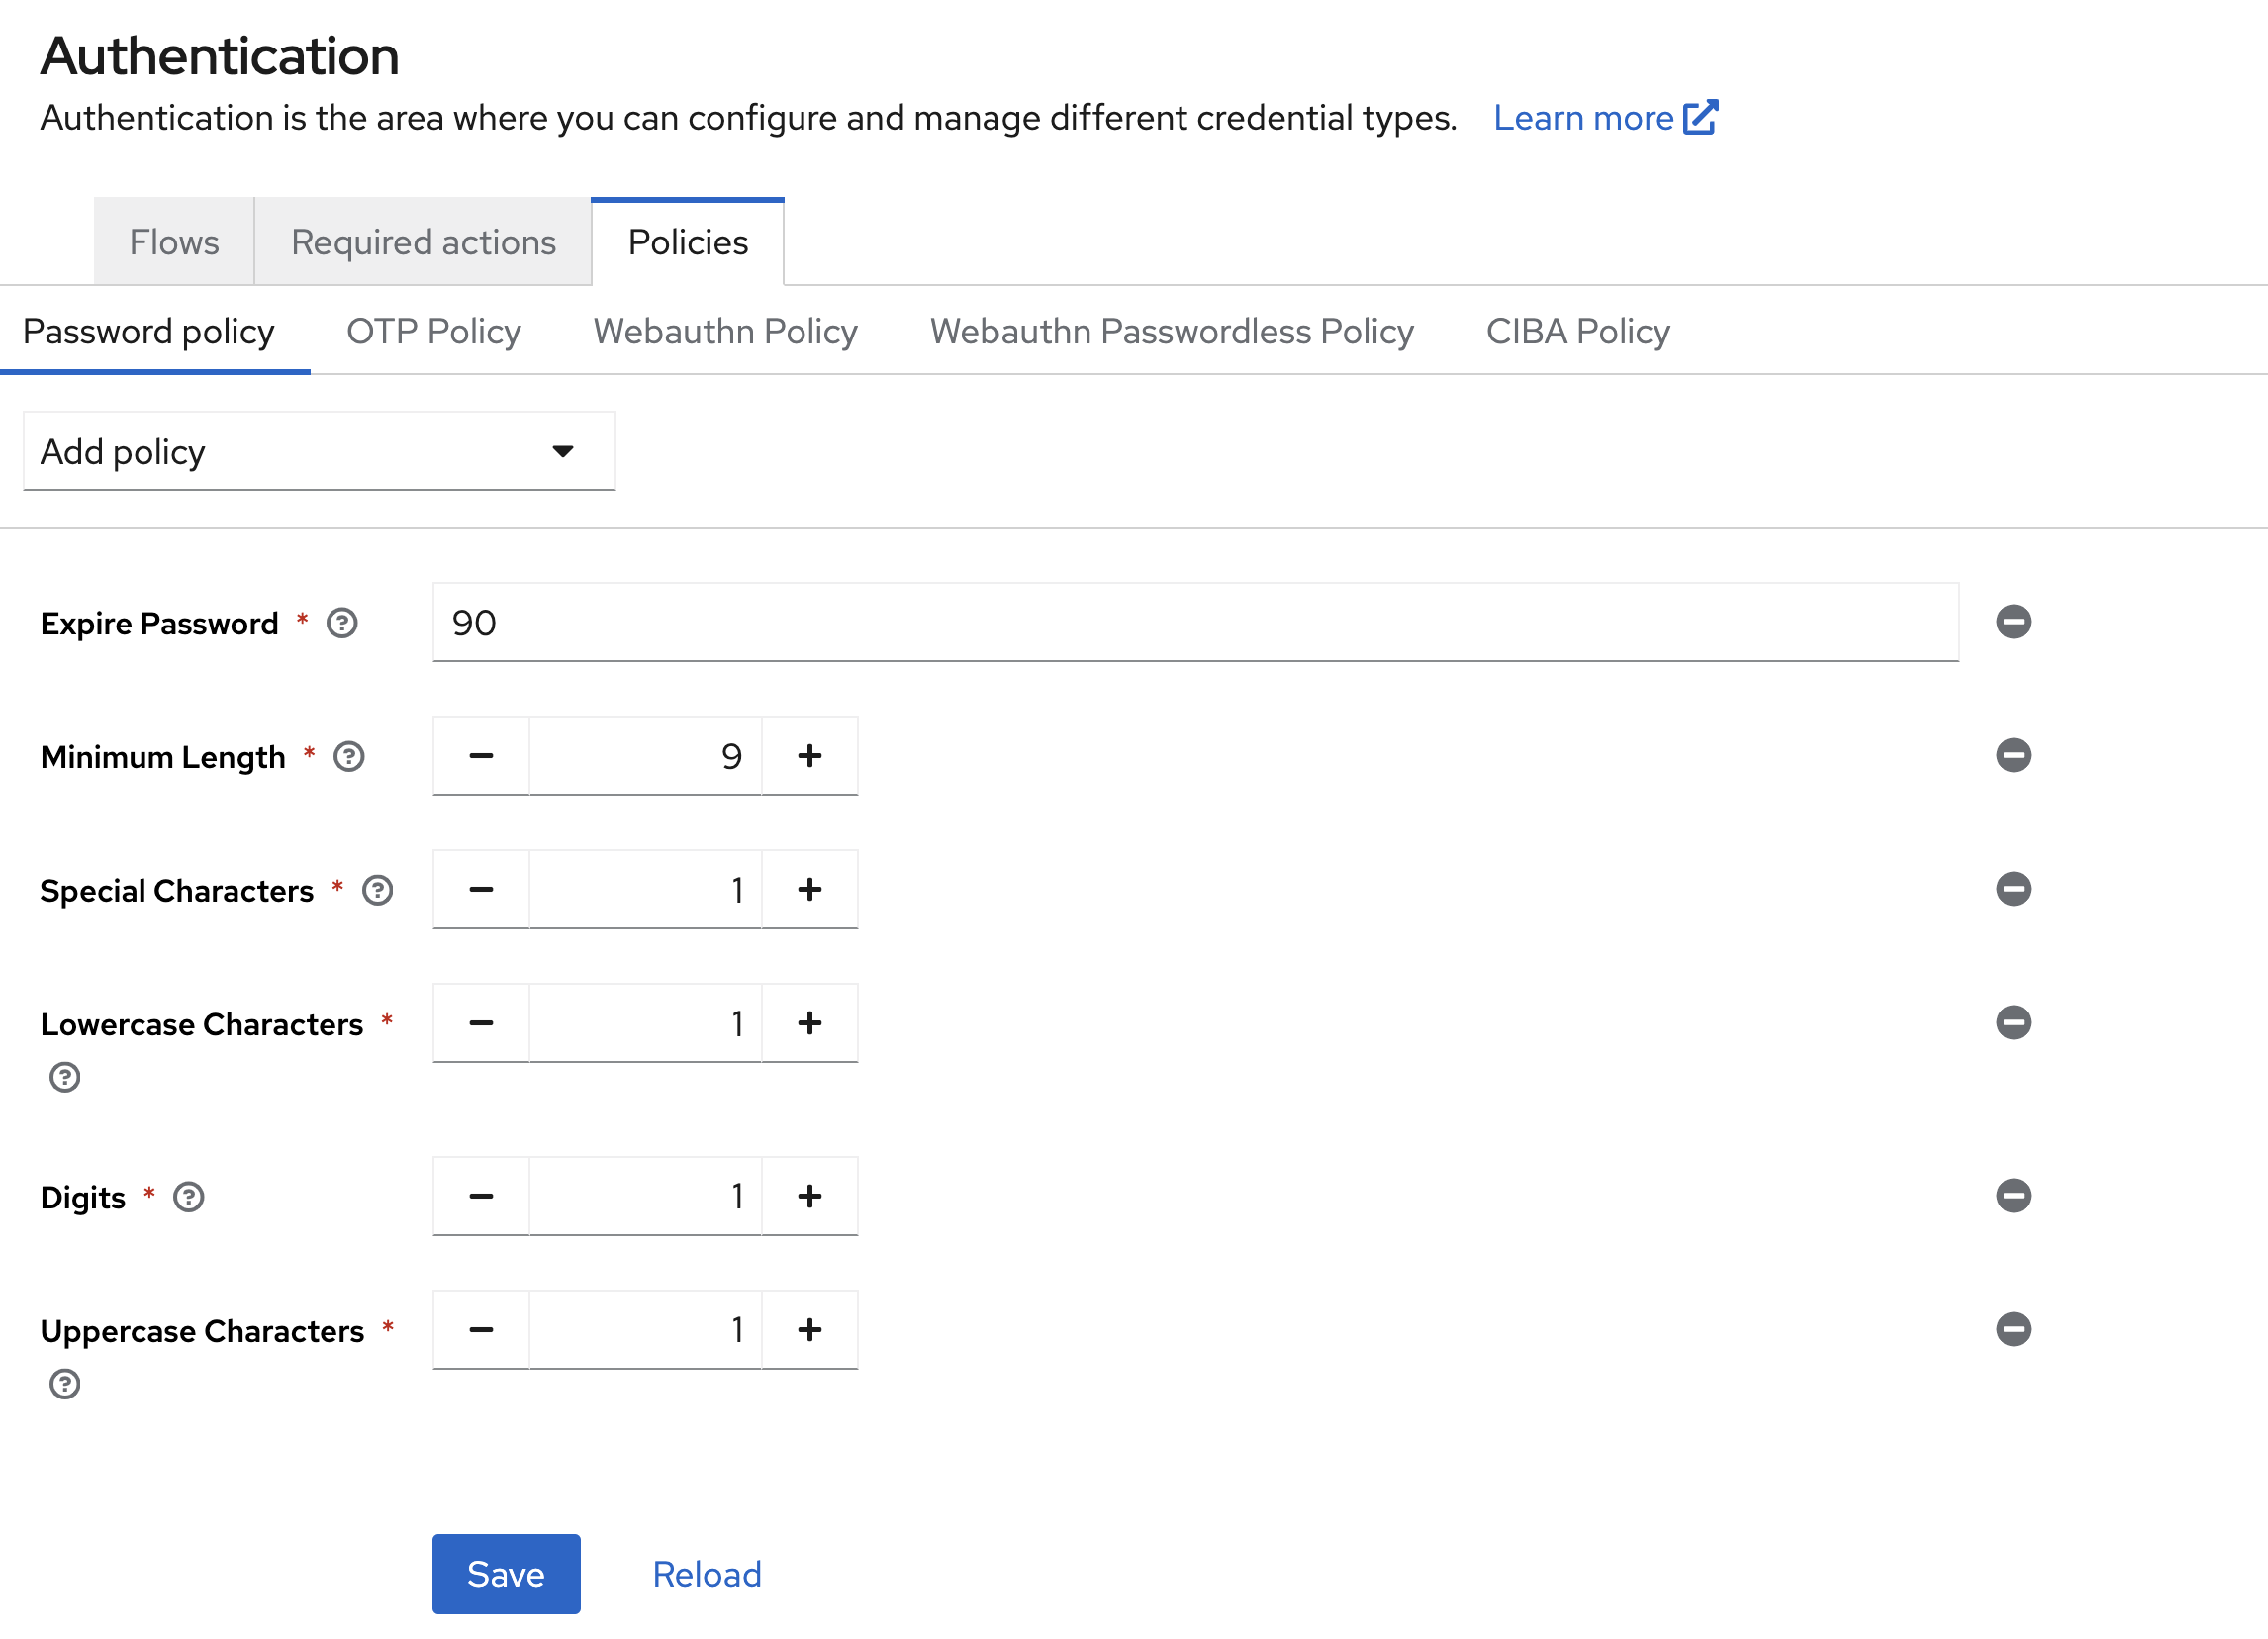
\includegraphics[width=0.5\textwidth]{contents/contents/image_16.png}
    \caption{Password policy cho người dùng}
    \label{fig:example_image}
    
\end{figure}

\subsection{Tích hợp Keycloak vào Cloudflare Zero Trust}
Ở bước này, Keycloak được khai báo như một nhà cung cấp danh tính OIDC cho hệ thống Cloudflare Zero Trust.
\begin{itemize}
    \item Truy cập mục quản lý Identity Providers trong Cloudflare Zero Trust và chọn thêm nhà cung cấp OIDC tùy chỉnh.
    \item Điền các tham số tích hợp gồm \textit{client ID}, \textit{client secret}, \textit{issuer URL} và các endpoint tương ứng lấy từ Keycloak qua tunnel công khai.
    \item Kiểm tra quá trình đồng bộ thông tin định danh để bảo đảm Cloudflare có thể chuyển hướng người dùng tới Keycloak và nhận lại token hợp lệ.
    \item Xác nhận các trường nhận dạng như email, username hoặc nhóm người dùng có thể được dùng làm điều kiện trong Access Policy.
\end{itemize}
\begin{figure}[H]
    \centering
    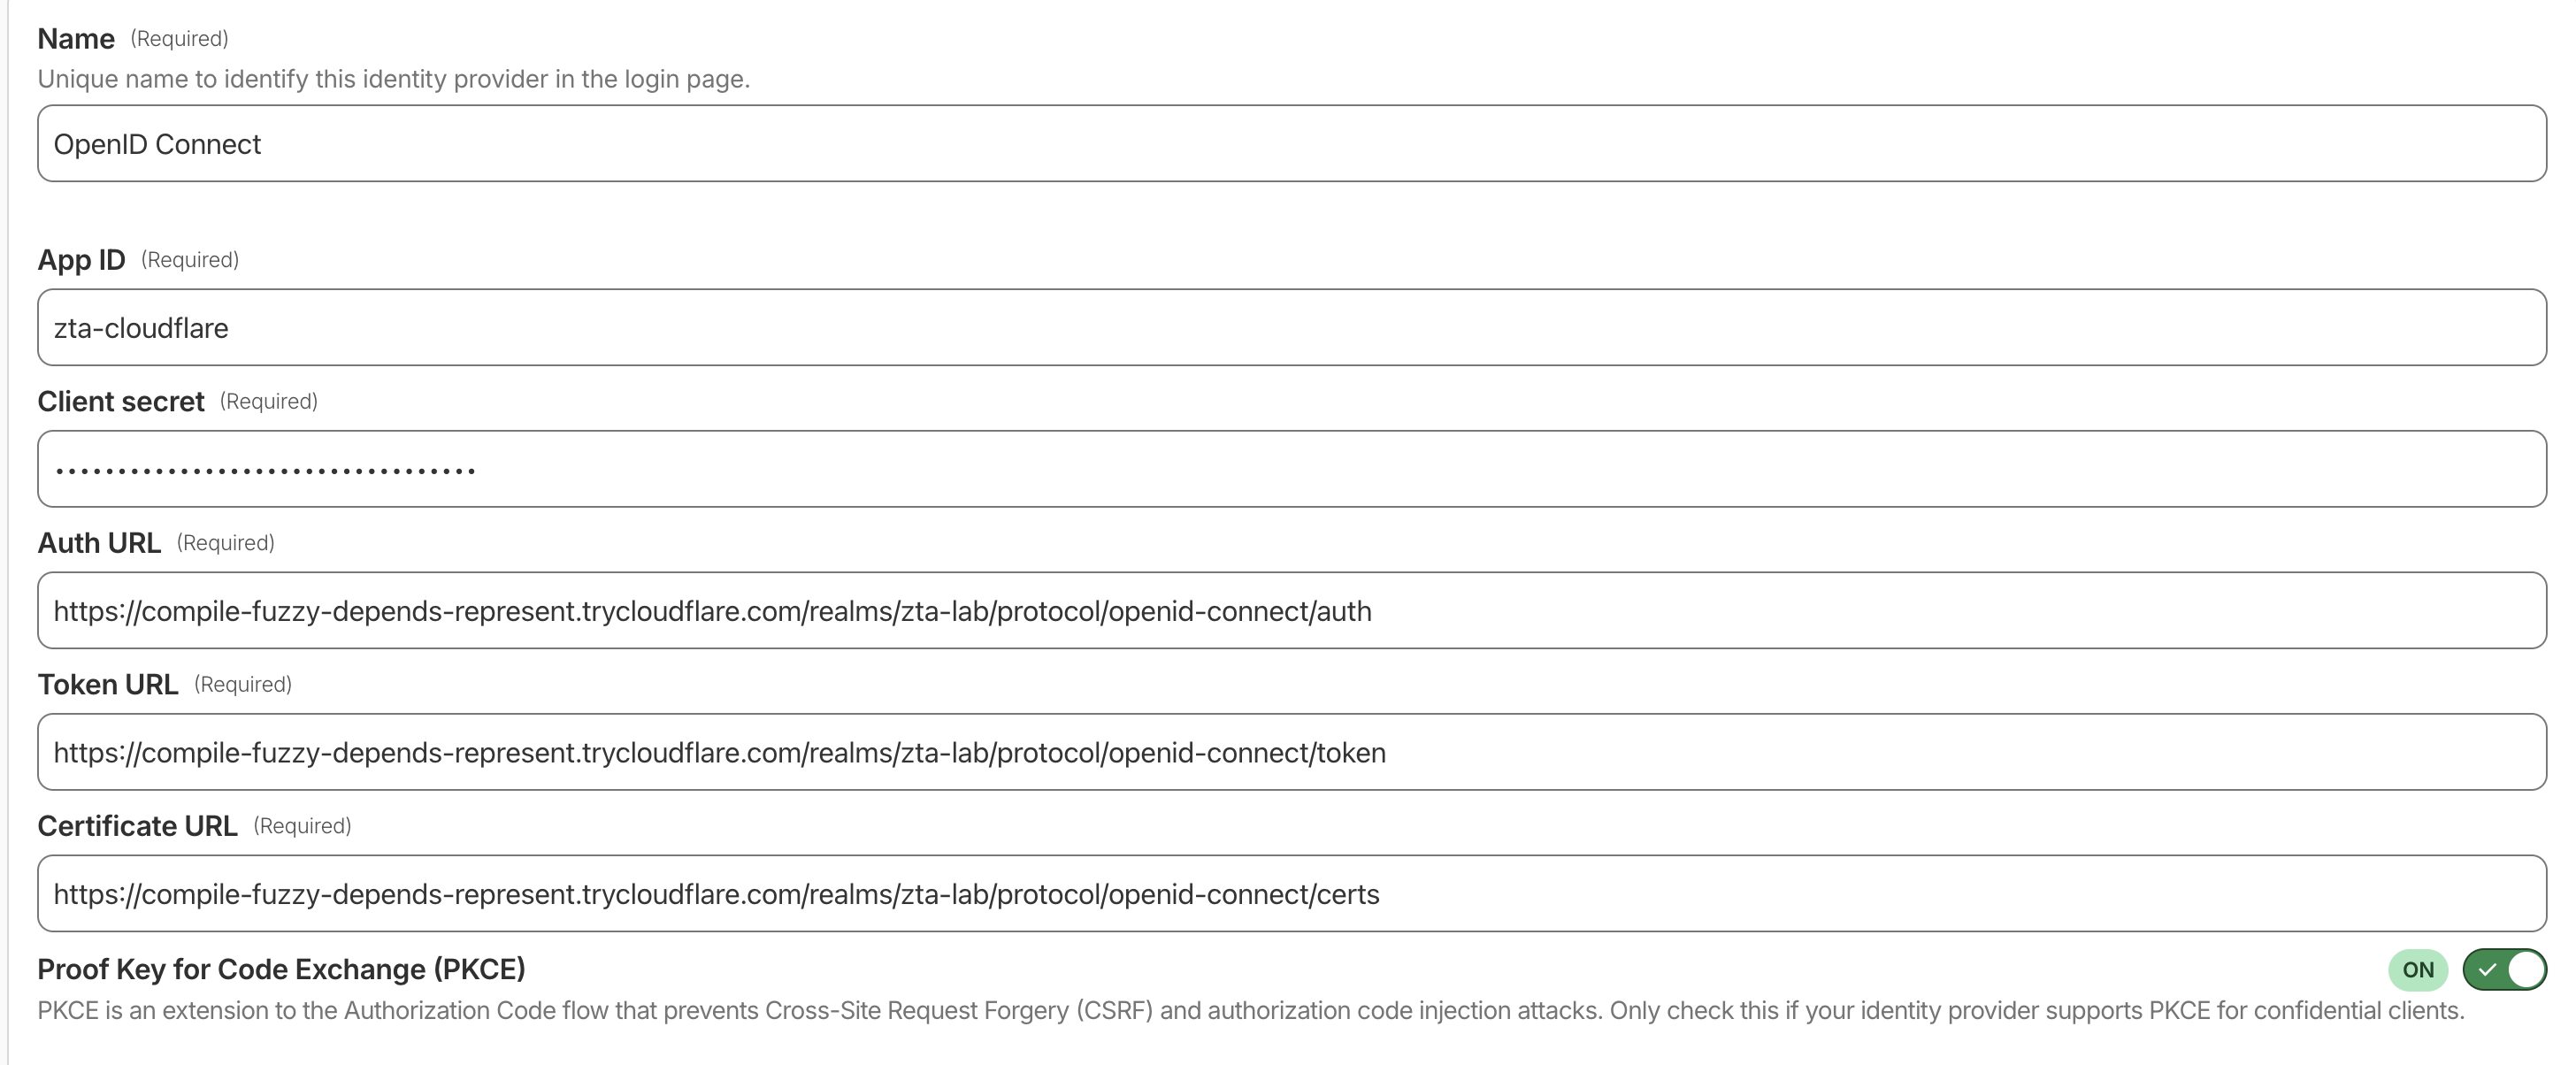
\includegraphics[width=0.5\textwidth]{contents/contents/image_6.png}
    \caption{Cấu hình IdP cho Cloudflare Zero Trust}
    \label{fig:example_image}
    
\end{figure}

\subsection{Xây dựng Access Policies cho các route bên trong app}
Sau khi hoàn tất liên kết định danh, hệ thống tiếp tục được ràng buộc bởi các chính sách truy cập theo nguyên tắc đặc quyền tối thiểu.
\begin{itemize}
    \item Tạo ứng dụng được bảo vệ trong Cloudflare Access, gắn với hostname hoặc đường dẫn cần kiểm soát.
    \item Khai báo chính sách \textbf{Allow} dựa trên danh tính người dùng, email, nhóm hoặc vai trò nhận được từ Keycloak.
    \item Bổ sung các điều kiện ngữ cảnh như quốc gia, địa chỉ IP hoặc yêu cầu xác thực lại khi cần để tăng mức độ bảo vệ.
    \item Thiết lập thứ tự ưu tiên giữa các chính sách \textbf{Allow}, \textbf{Deny} và \textbf{Bypass} để tránh xung đột trong quá trình đánh giá quyền truy cập.
    \item Một số policy được áp dụng: 
\end{itemize}

\begin{figure}[H]
    \centering
    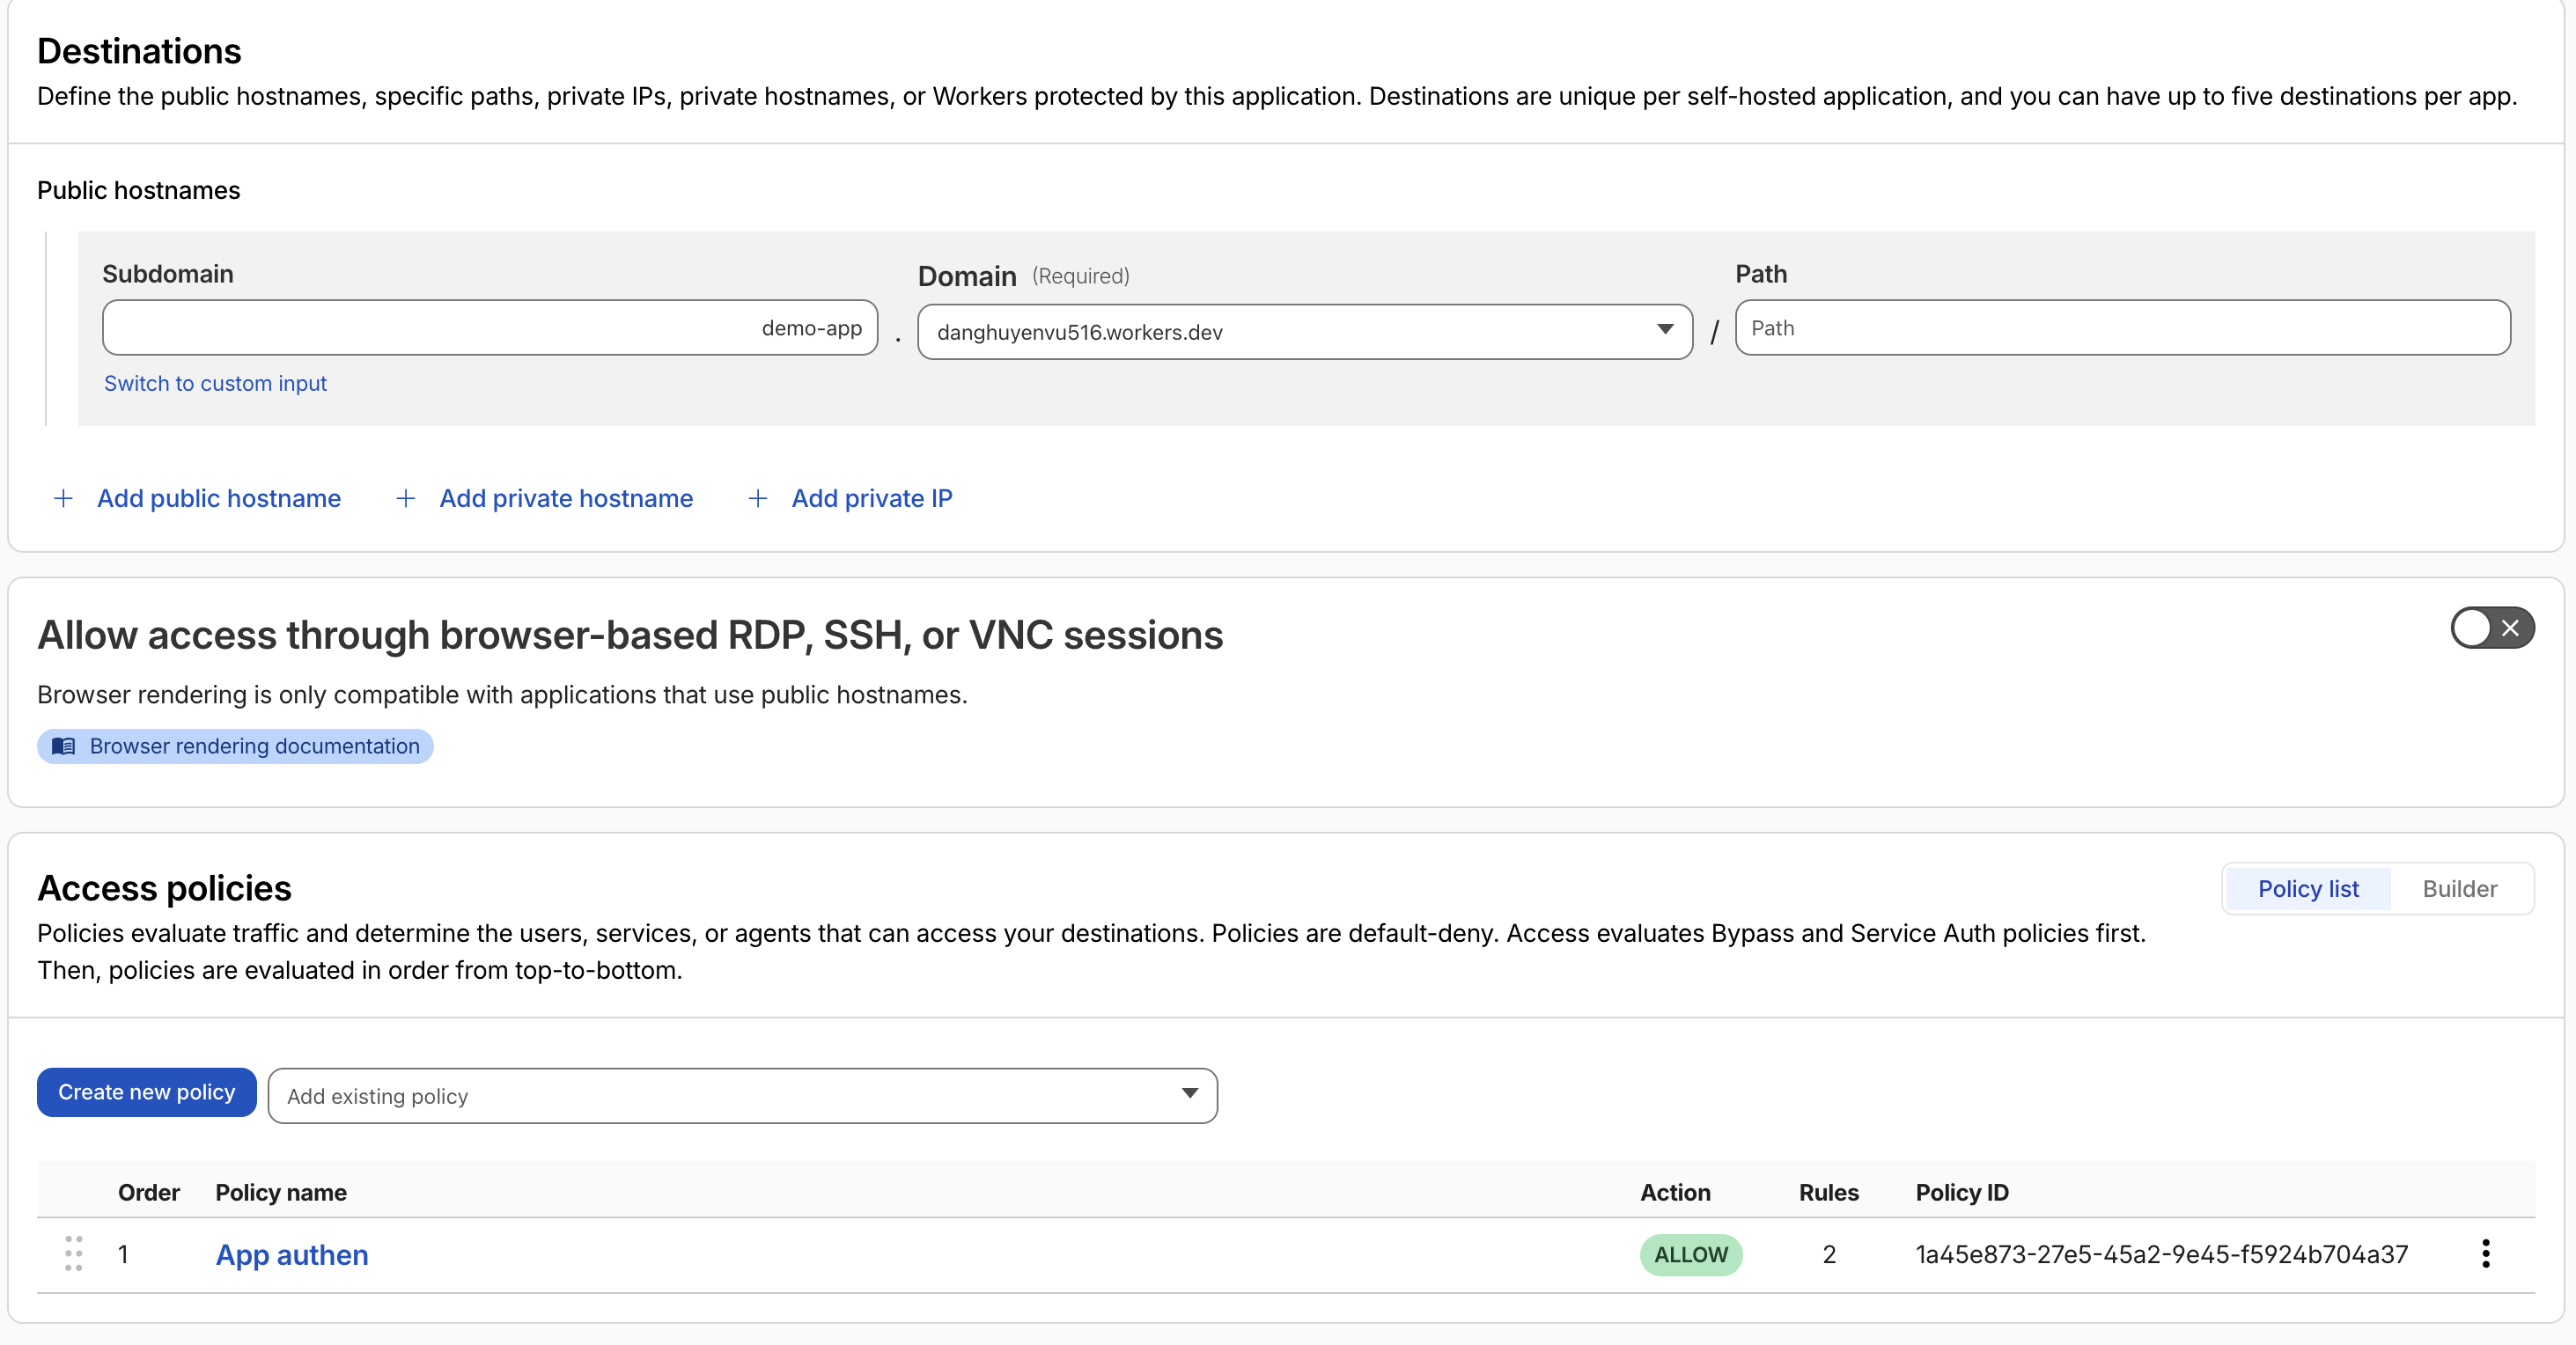
\includegraphics[width=0.5\textwidth]{contents/contents/image_12.png}
    \caption{Access policy cho Protected Application yêu cầu xác thực qua IdP}
    \label{fig:example_image}
    
\end{figure}

\begin{figure}[H]
    \centering
    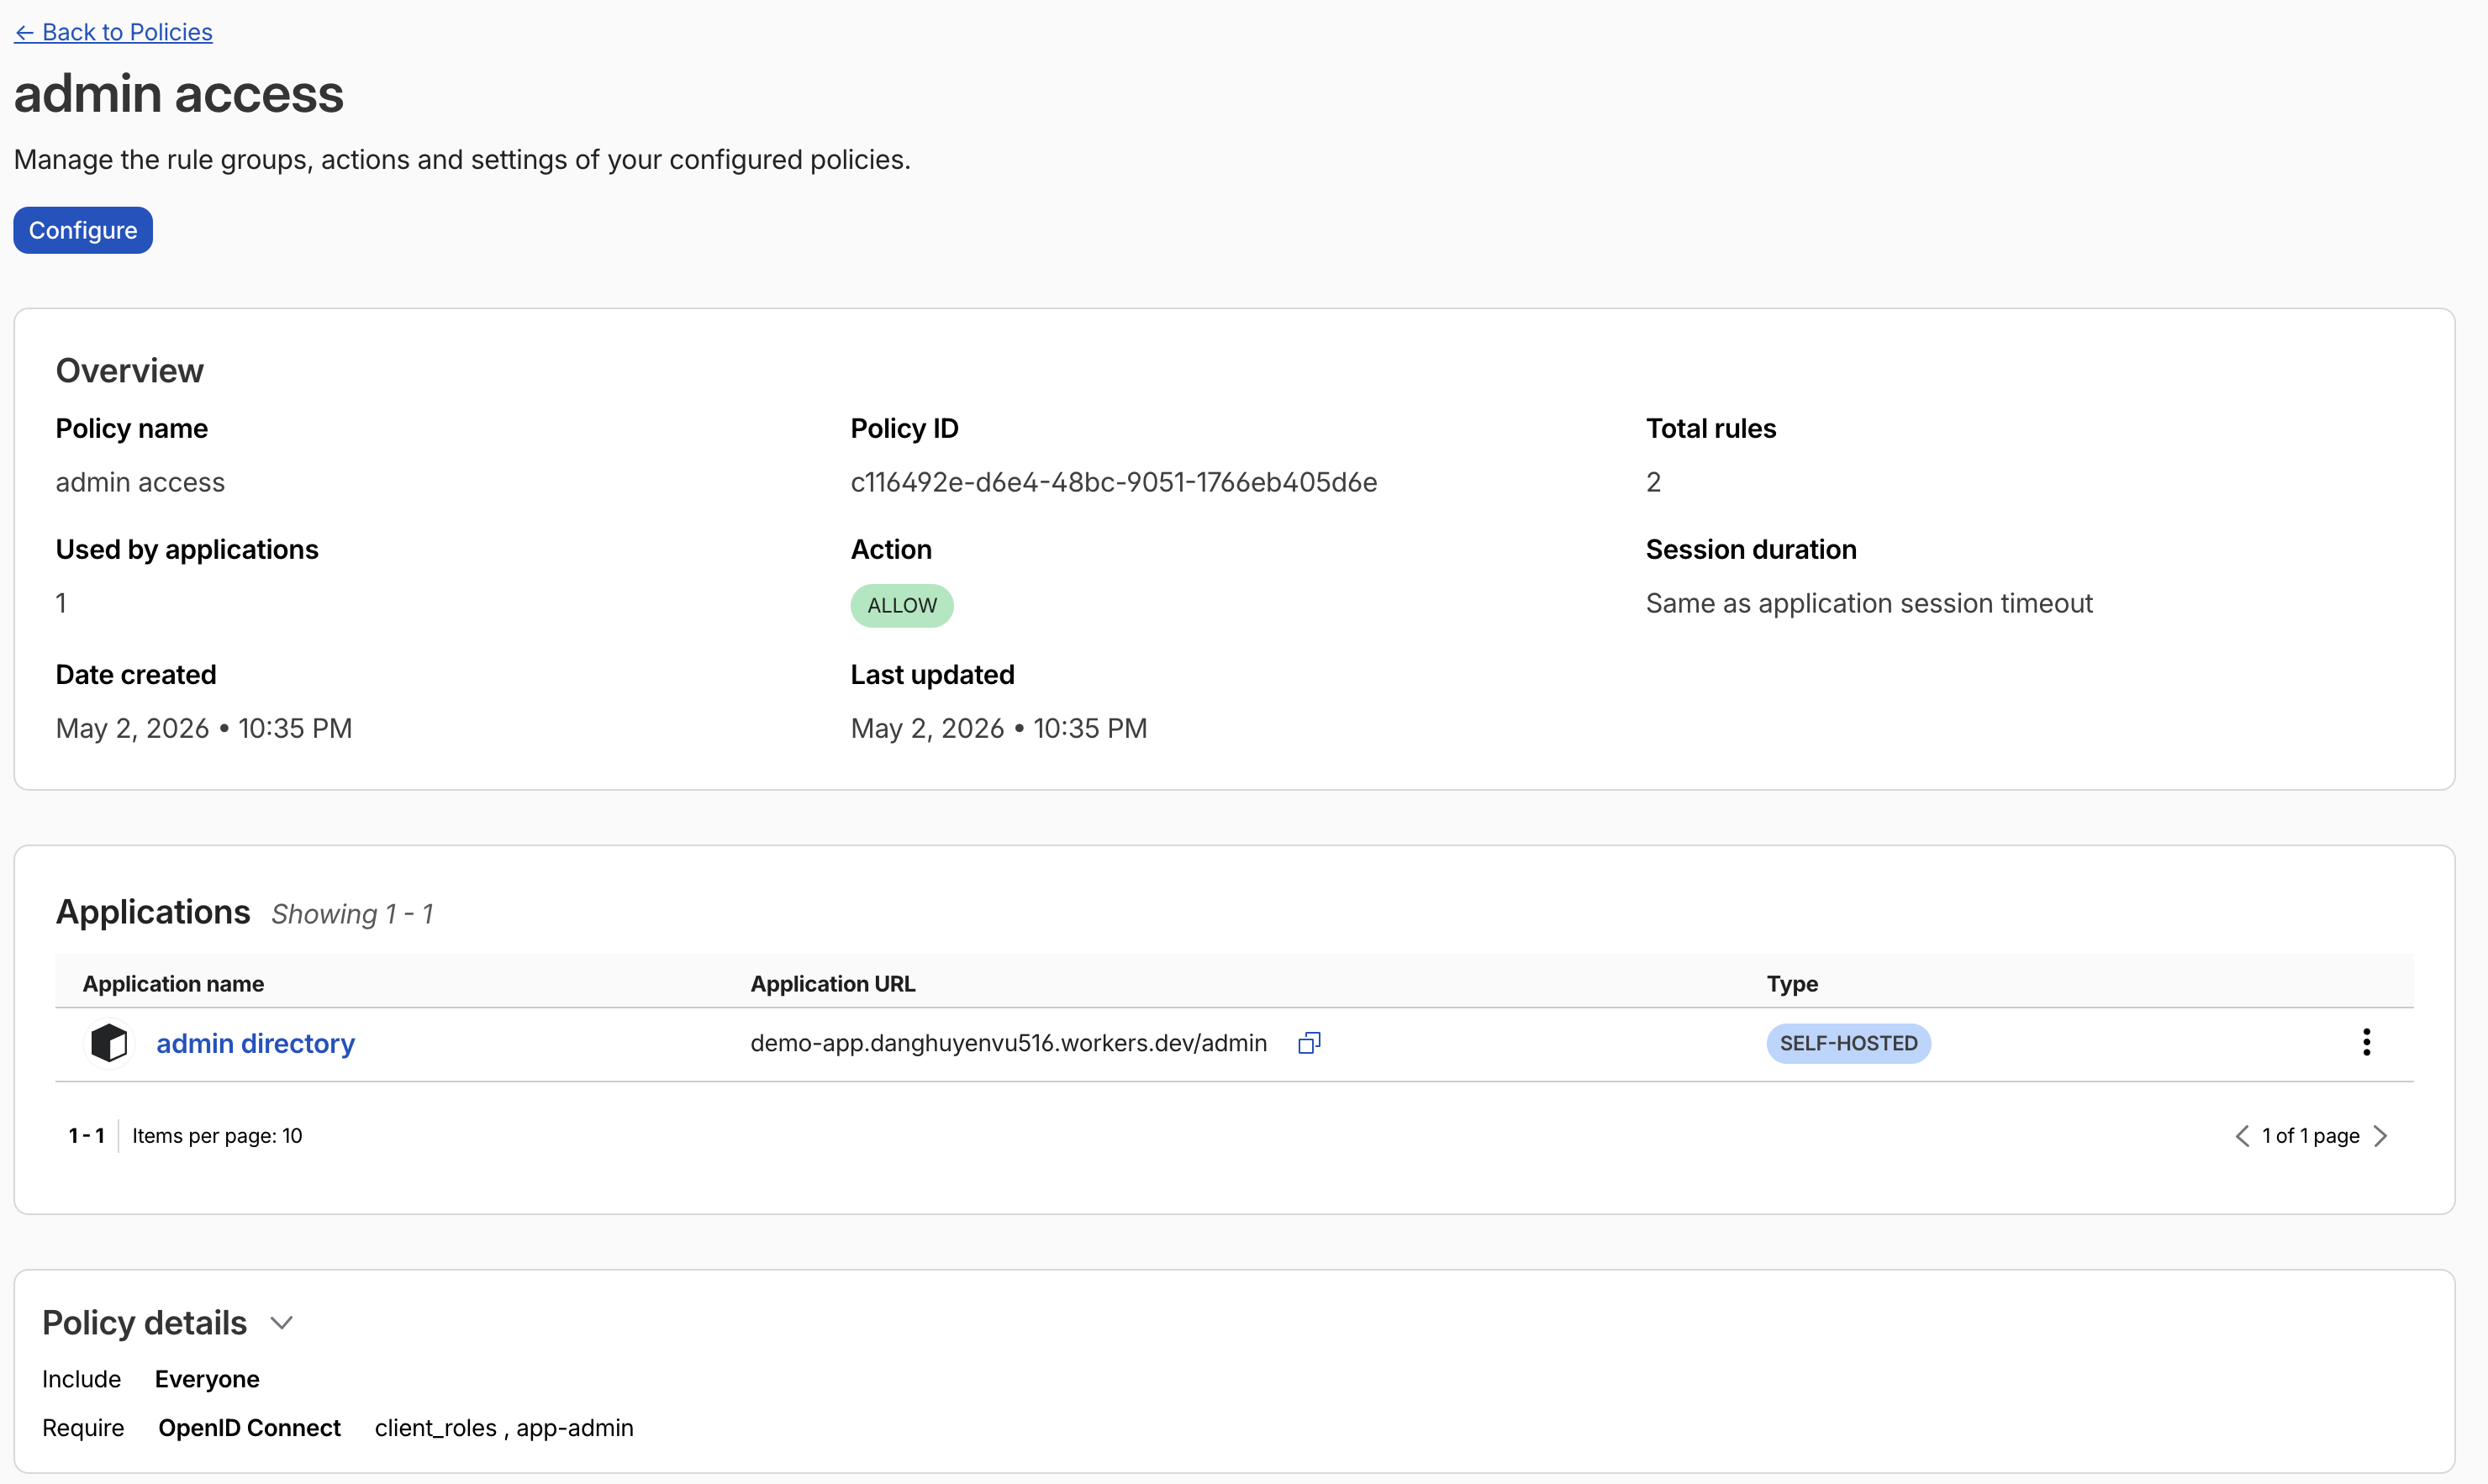
\includegraphics[width=0.5\textwidth]{contents/contents/image_19.png}
    \caption{Policy kiểm soát truy cập tài nguyên của admin}
    \label{fig:example_image}
    
\end{figure}

\begin{figure}[H]
    \centering
    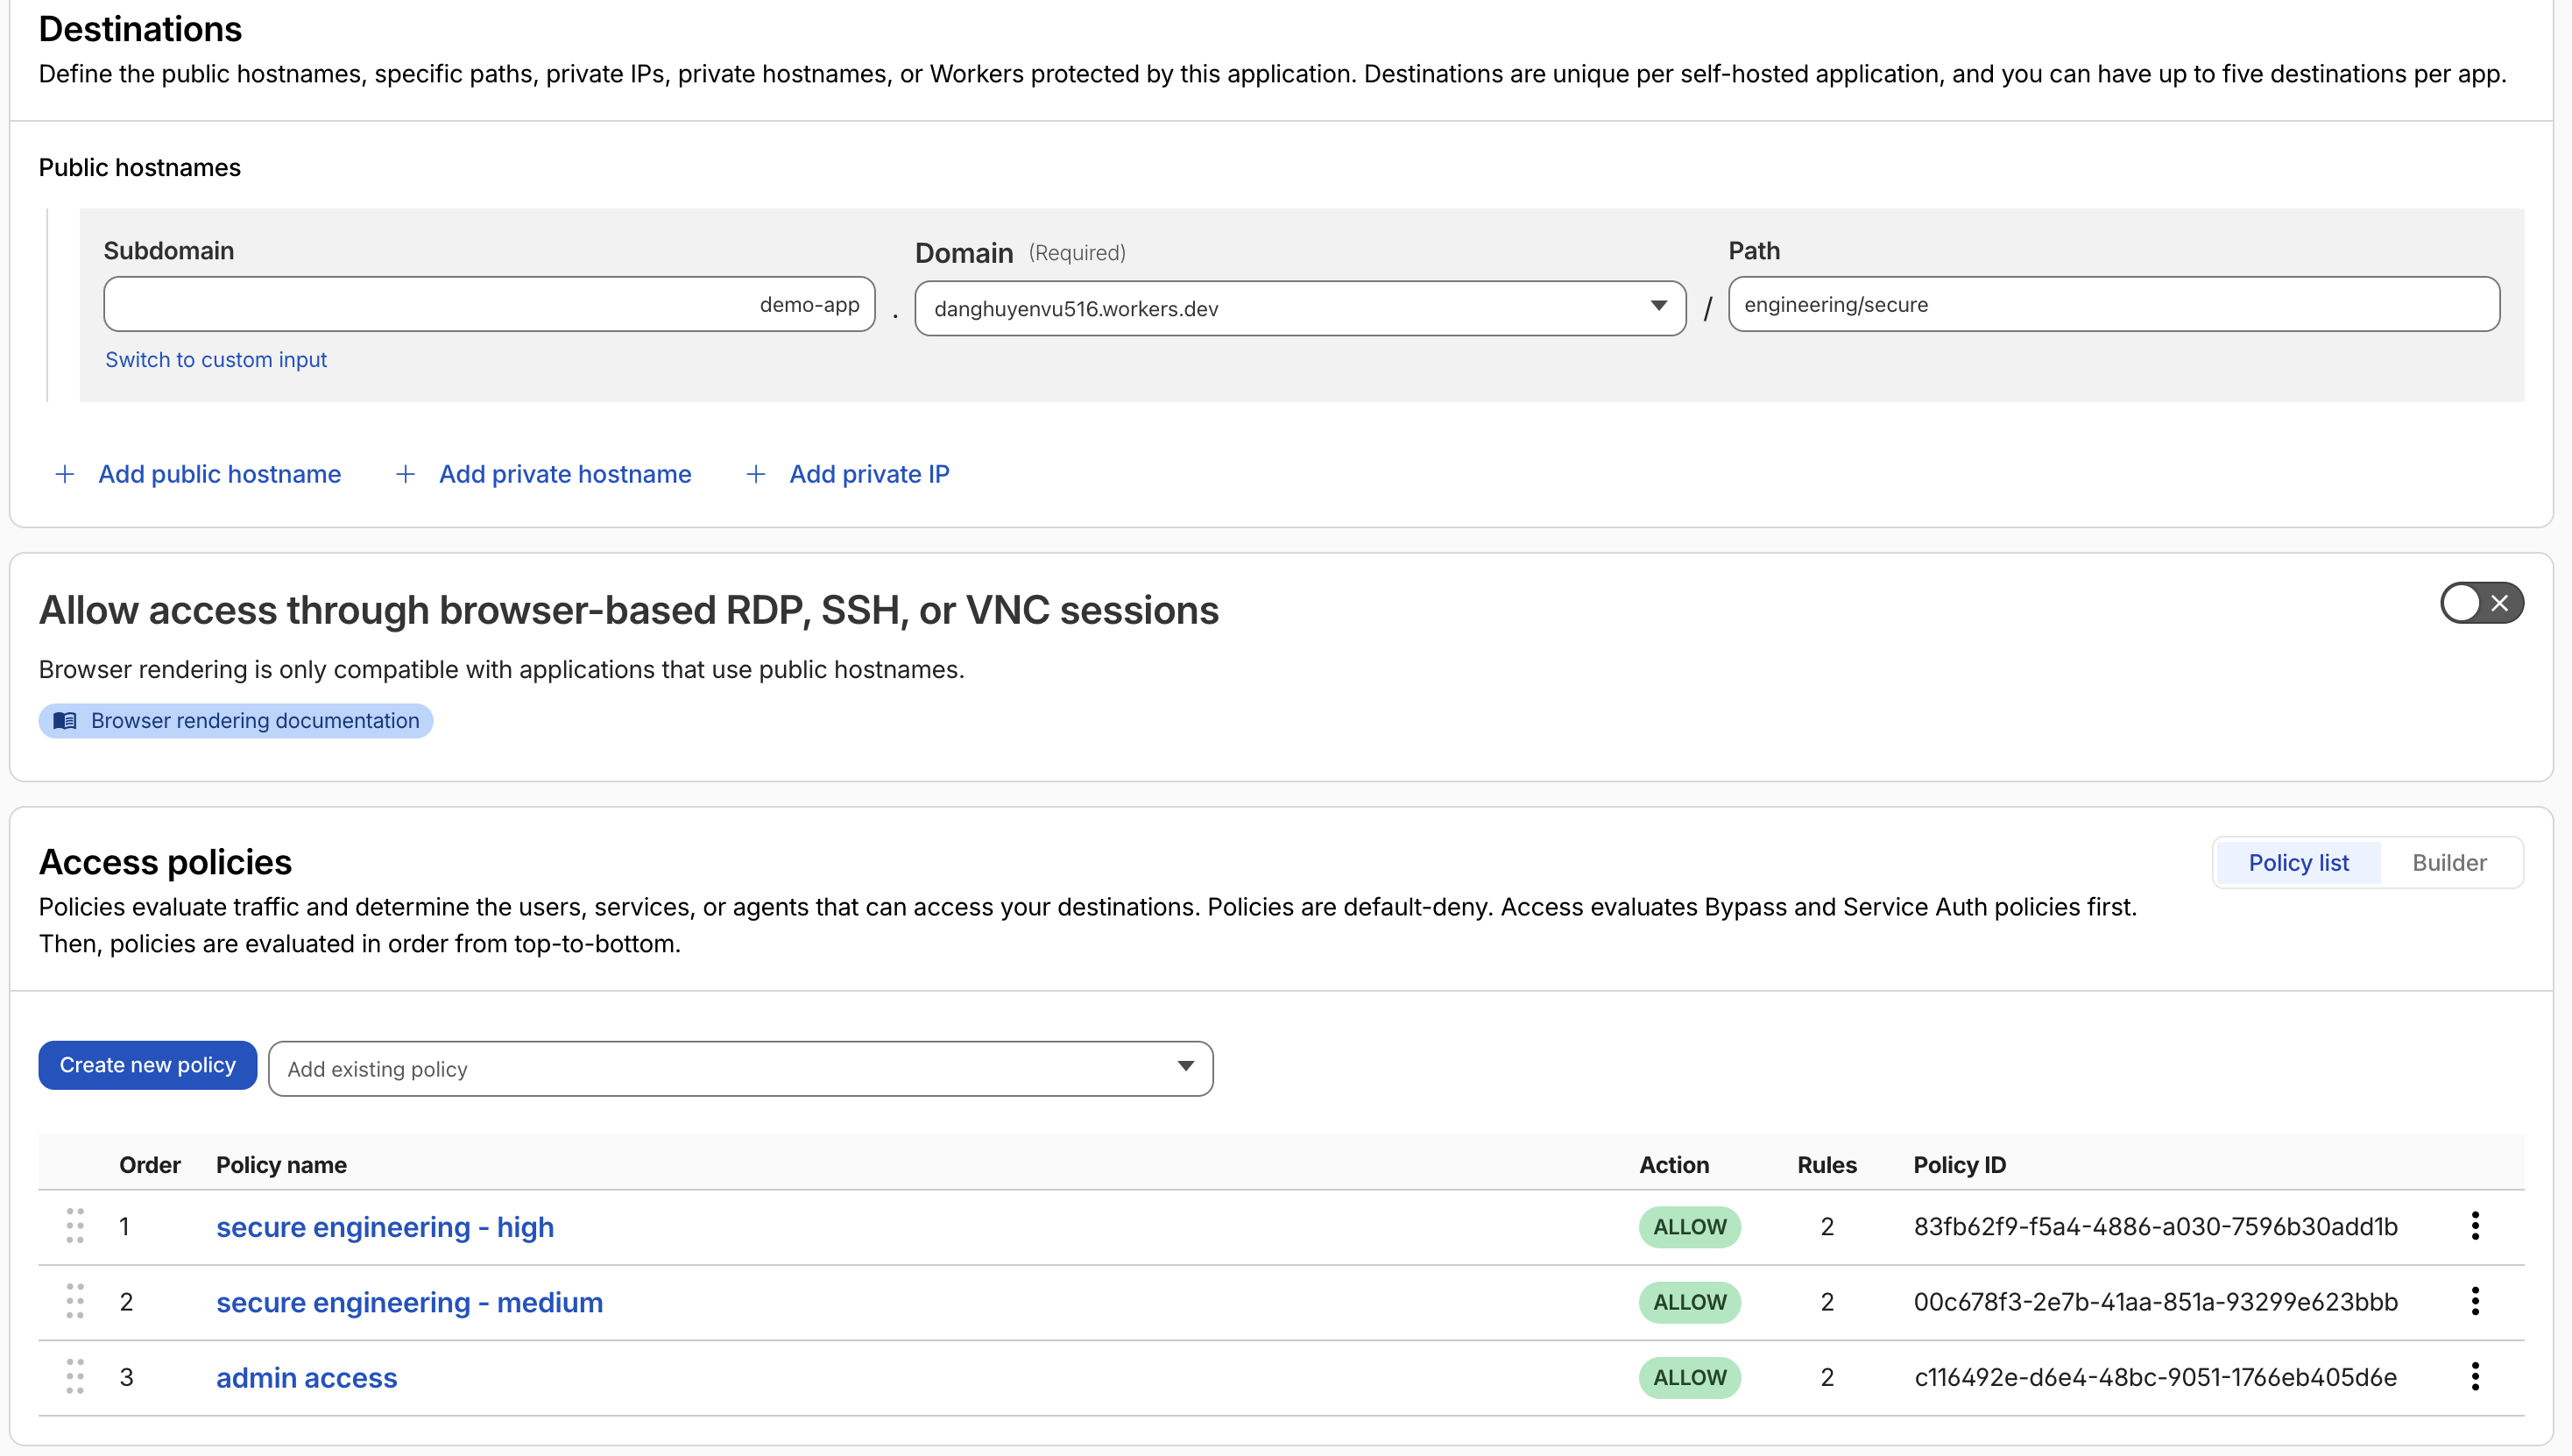
\includegraphics[width=0.5\textwidth]{contents/contents/image_20.png}
    \caption{Áp dụng policy cho /engineering/secure yêu cầu khắt khe hơn khi truy cập những tài nguyên quan trọng}
    \label{fig:example_image}
    
\end{figure}

\subsection{Kiểm thử luồng đăng nhập}
Luồng kiểm thử được thực hiện từ góc nhìn người dùng cuối nhằm xác nhận toàn bộ chuỗi xác thực và ủy quyền hoạt động đúng như thiết kế.
\begin{figure}[H]
    \centering
    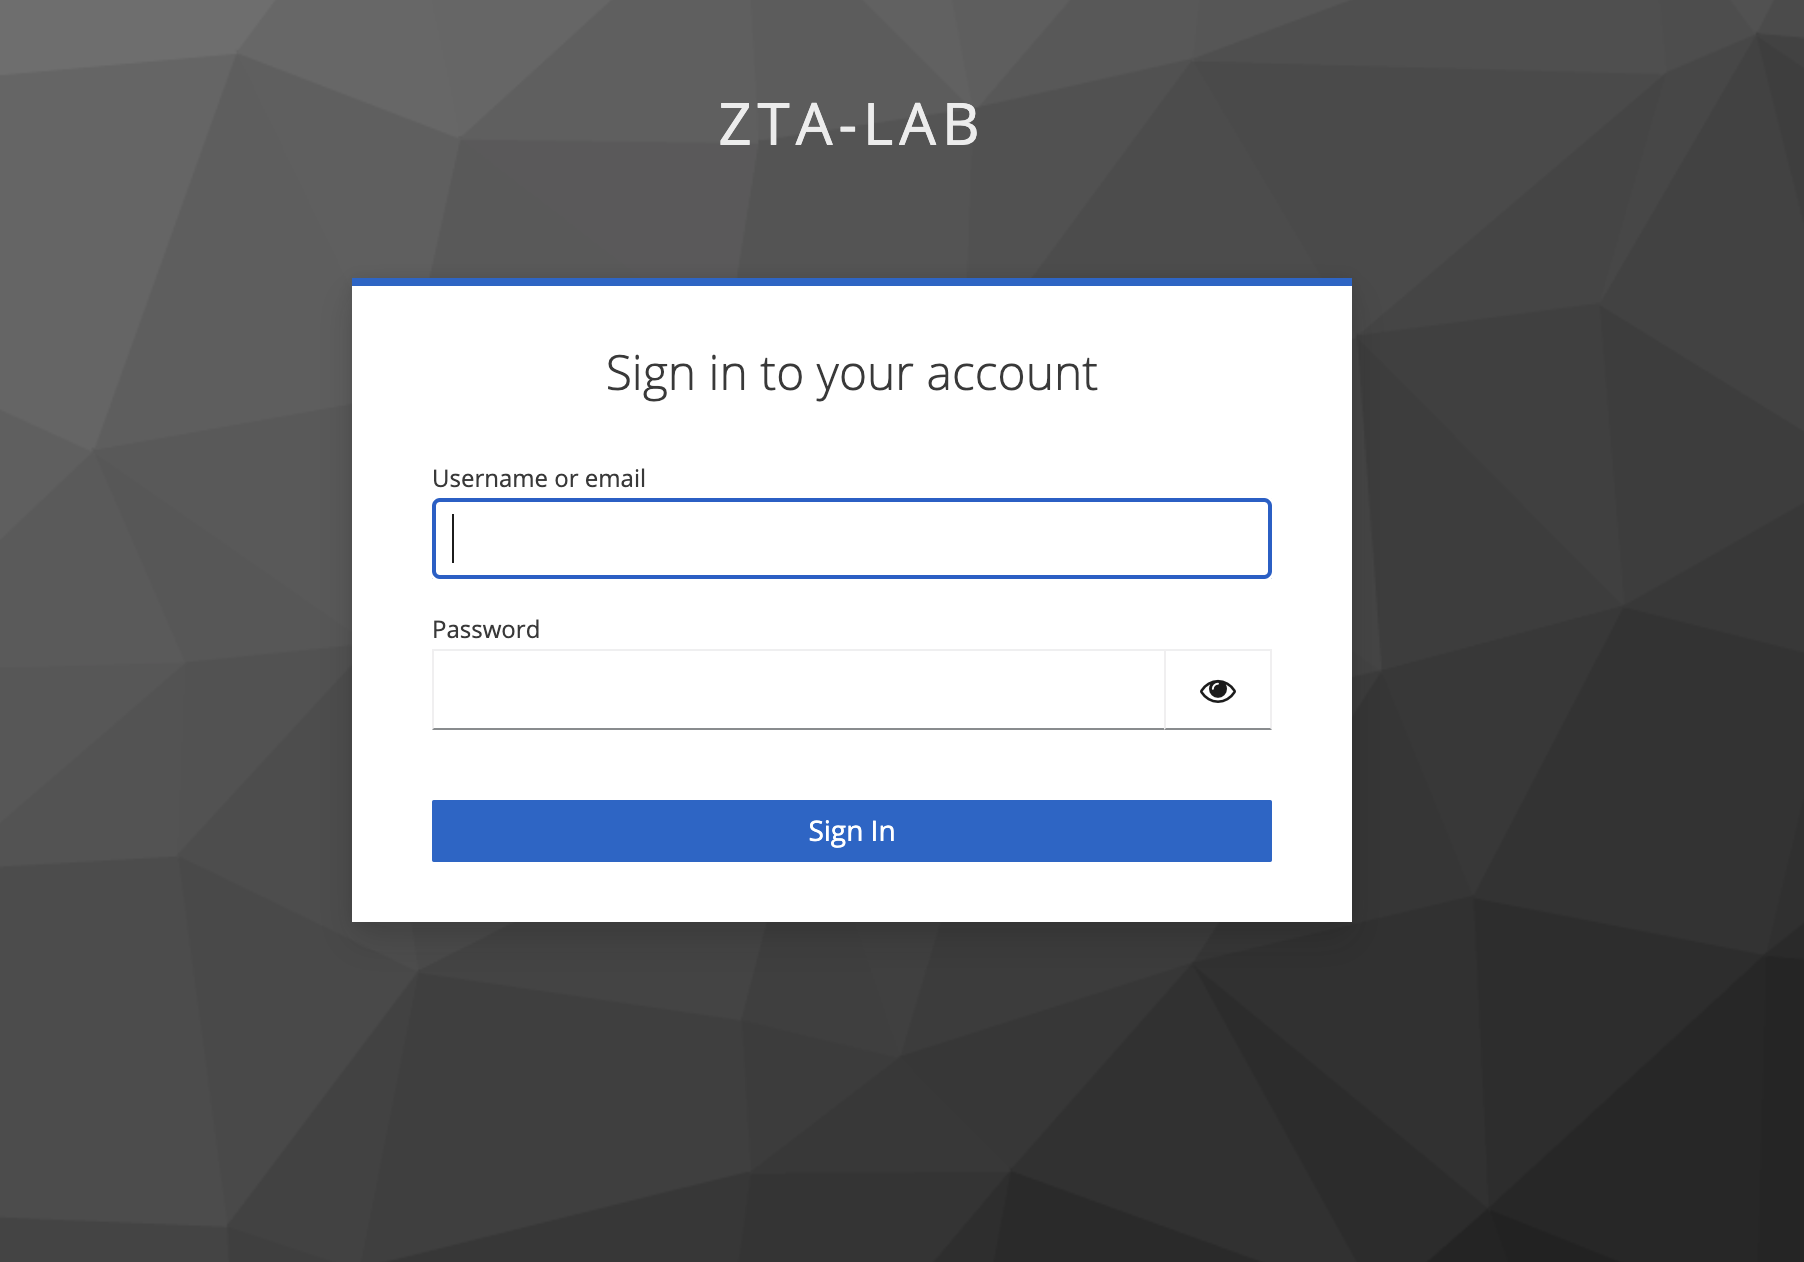
\includegraphics[width=0.5\textwidth]{contents/contents/image_13.png}
    \caption{Login page của Keycloak}
    \label{fig:example_image}
\end{figure}
Người dùng khi muốn truy cập ứng dụng web được bảo vệ nếu chưa được xác thực sẽ bị Cloudflare Access chặn lại tại lớp biên và điều hướng tới trang login của Keycloak để xác thực thông qua giao thức OIDC.

\begin{figure}[h]
    \centering
    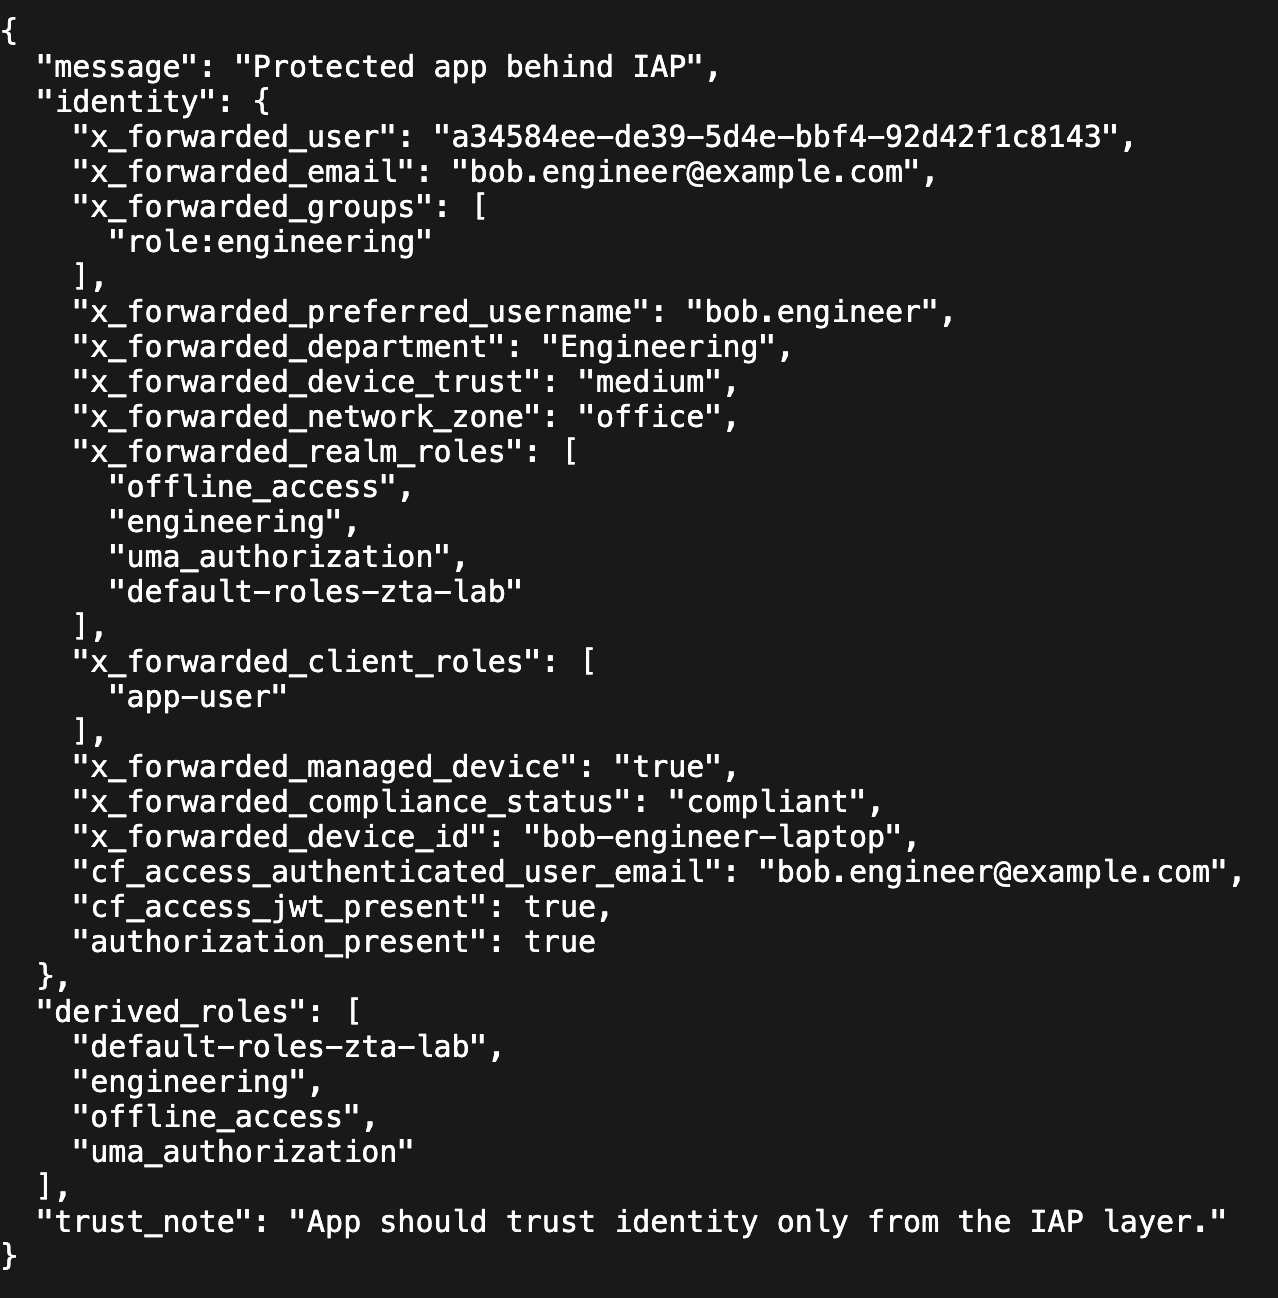
\includegraphics[width=0.5\textwidth]{contents/contents/image_14.png}
    \caption{Thông tin user khi đăng nhập thành công}
    \label{fig:example_image}
    
\end{figure}

Một người dùng muốn truy cập các tài nguyên không được phép sẽ bị chặn:
\begin{figure}[H]
    \centering
    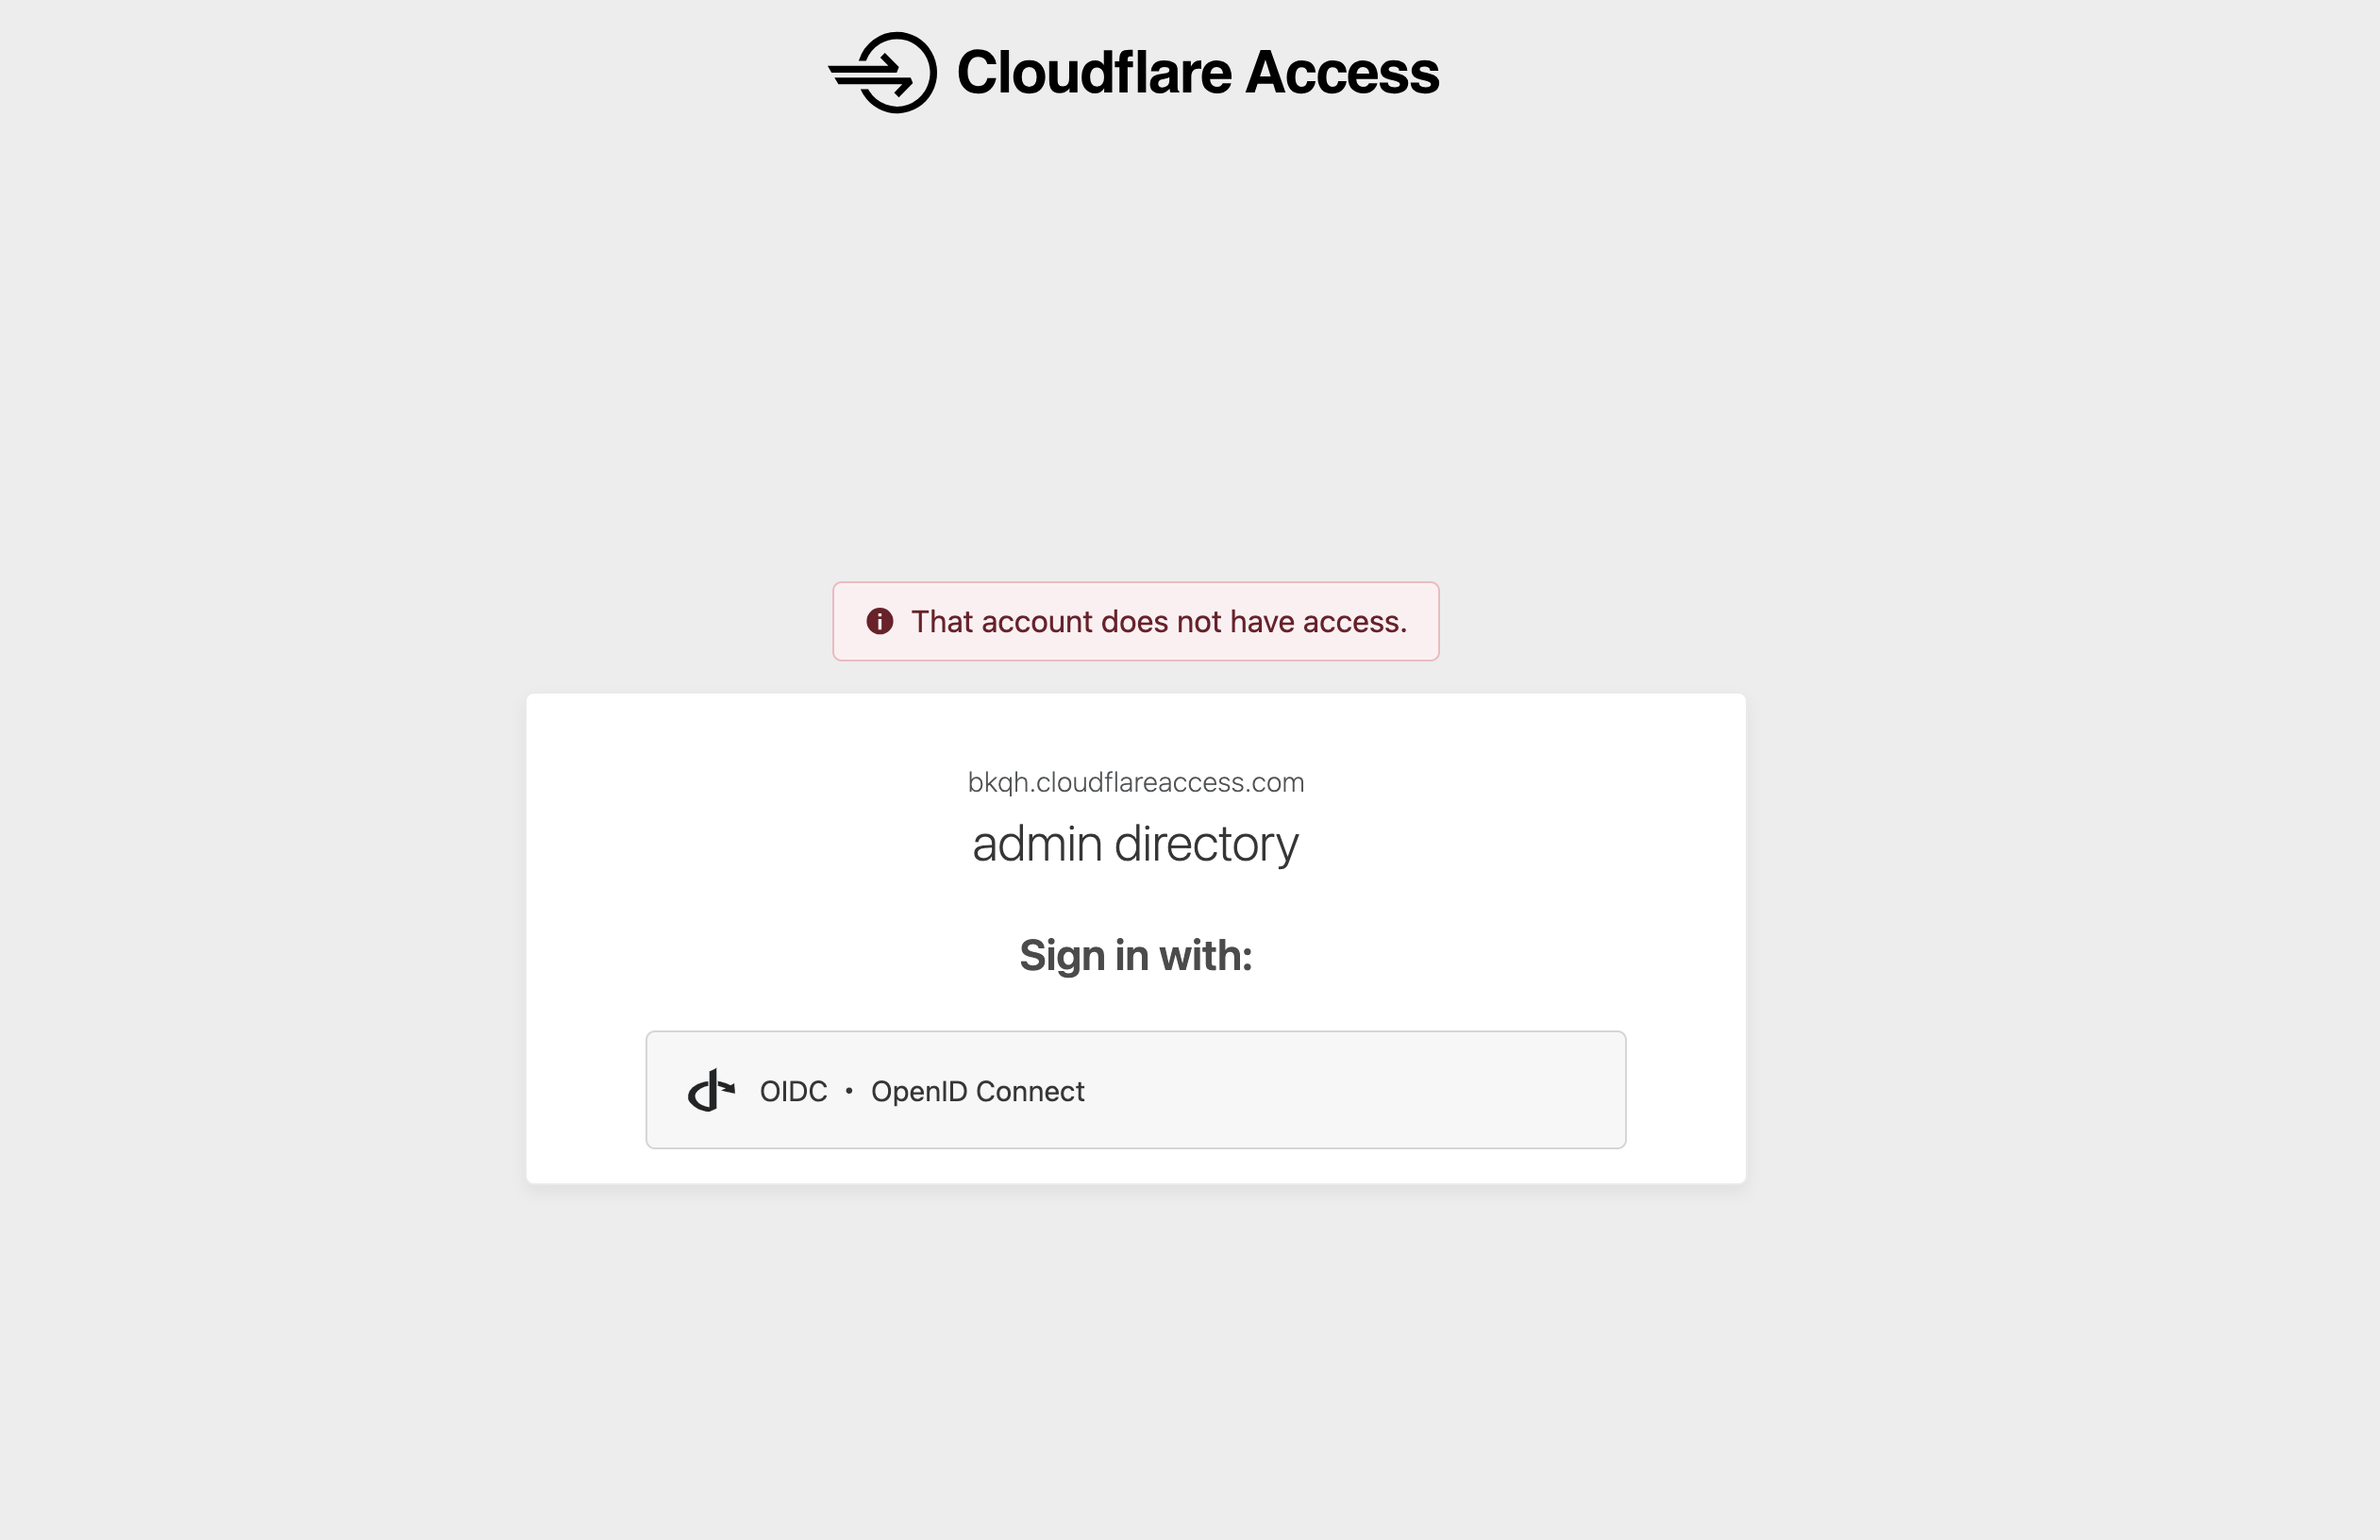
\includegraphics[width=0.5\textwidth]{contents/contents/image_18.png}
    \caption{Người dùng không đủ đặc quyền bị chặn khi truy cập directory yêu cầu đặc quyền cao với claim tương ứng}
    \label{fig:example_image}
    
\end{figure}

\begin{itemize}
    \item Người dùng truy cập ứng dụng được bảo vệ và bị Cloudflare Access chặn tại lớp biên.
    \item Cloudflare chuyển hướng người dùng sang trang đăng nhập Keycloak thông qua giao thức OIDC.
    \item Sau khi xác thực thành công, Keycloak trả mã hoặc token cho Cloudflare để hoàn tất phiên đăng nhập.
    \item Cloudflare đánh giá token cùng các Access Policies; nếu đạt điều kiện thì cấp quyền vào ứng dụng, ngược lại từ chối truy cập.
\end{itemize}

\subsection{Định hướng đánh giá}
Phần đánh giá tập trung vào cả tính đúng đắn của luồng xác thực lẫn hiệu quả bảo vệ tài nguyên.
\begin{itemize}
    \item \textbf{Đánh giá chức năng}: Kiểm tra khả năng đăng nhập thành công với người dùng hợp lệ và từ chối với người dùng không thuộc chính sách.
    \item \textbf{Đánh giá bảo mật}: Xem xét việc ẩn IP gốc nhờ Tunnel, khả năng chặn truy cập trực tiếp và hiệu quả của kiểm soát theo danh tính.
    \item \textbf{Đánh giá vận hành}: Ghi nhận độ thuận tiện khi cấu hình thử nghiệm bằng \texttt{trycloudflare}, đồng thời chỉ ra hạn chế của tunnel miễn phí trong triển khai dài hạn.
    \item \textbf{Đánh giá trải nghiệm}: Quan sát số bước đăng nhập, độ trễ chuyển hướng và tính minh bạch của luồng xác thực đối với người dùng cuối.
\end{itemize}
